\documentclass{report}\usepackage[]{graphicx}\usepackage[]{color}
% maxwidth is the original width if it is less than linewidth
% otherwise use linewidth (to make sure the graphics do not exceed the margin)
\makeatletter
\def\maxwidth{ %
  \ifdim\Gin@nat@width>\linewidth
    \linewidth
  \else
    \Gin@nat@width
  \fi
}
\makeatother

\definecolor{fgcolor}{rgb}{0.345, 0.345, 0.345}
\makeatletter
\@ifundefined{AddToHook}{}{\AddToHook{package/xcolor/after}{\definecolor{fgcolor}{rgb}{0.345, 0.345, 0.345}}}
\makeatother
\newcommand{\hlnum}[1]{\textcolor[rgb]{0.686,0.059,0.569}{#1}}%
\newcommand{\hlstr}[1]{\textcolor[rgb]{0.192,0.494,0.8}{#1}}%
\newcommand{\hlcom}[1]{\textcolor[rgb]{0.678,0.584,0.686}{\textit{#1}}}%
\newcommand{\hlopt}[1]{\textcolor[rgb]{0,0,0}{#1}}%
\newcommand{\hlstd}[1]{\textcolor[rgb]{0.345,0.345,0.345}{#1}}%
\newcommand{\hlkwa}[1]{\textcolor[rgb]{0.161,0.373,0.58}{\textbf{#1}}}%
\newcommand{\hlkwb}[1]{\textcolor[rgb]{0.69,0.353,0.396}{#1}}%
\newcommand{\hlkwc}[1]{\textcolor[rgb]{0.333,0.667,0.333}{#1}}%
\newcommand{\hlkwd}[1]{\textcolor[rgb]{0.737,0.353,0.396}{\textbf{#1}}}%
\let\hlipl\hlkwb

\usepackage{framed}
\makeatletter
\newenvironment{kframe}{%
 \def\at@end@of@kframe{}%
 \ifinner\ifhmode%
  \def\at@end@of@kframe{\end{minipage}}%
  \begin{minipage}{\columnwidth}%
 \fi\fi%
 \def\FrameCommand##1{\hskip\@totalleftmargin \hskip-\fboxsep
 \colorbox{shadecolor}{##1}\hskip-\fboxsep
     % There is no \\@totalrightmargin, so:
     \hskip-\linewidth \hskip-\@totalleftmargin \hskip\columnwidth}%
 \MakeFramed {\advance\hsize-\width
   \@totalleftmargin\z@ \linewidth\hsize
   \@setminipage}}%
 {\par\unskip\endMakeFramed%
 \at@end@of@kframe}
\makeatother

\definecolor{shadecolor}{rgb}{.97, .97, .97}
\definecolor{messagecolor}{rgb}{0, 0, 0}
\definecolor{warningcolor}{rgb}{1, 0, 1}
\definecolor{errorcolor}{rgb}{1, 0, 0}
\makeatletter
\@ifundefined{AddToHook}{}{\AddToHook{package/xcolor/after}{
\definecolor{shadecolor}{rgb}{.97, .97, .97}
\definecolor{messagecolor}{rgb}{0, 0, 0}
\definecolor{warningcolor}{rgb}{1, 0, 1}
\definecolor{errorcolor}{rgb}{1, 0, 0}
}}
\makeatother
\newenvironment{knitrout}{}{} % an empty environment to be redefined in TeX

\usepackage{alltt}

\usepackage[usenames,dvipsnames,svgnames,table]{xcolor}

\usepackage[colorlinks=true,linkcolor=SteelBlue]{hyperref}

% set margins
\usepackage[margin=1in, headheight=3pt]{geometry}
%\geometry{left = 1in, right = 1in, top = 1in, bottom = 1in}

% set sof table figure
\usepackage{graphicx}
\usepackage{booktabs}
\usepackage{tabularx}
% \usepackage[T1]{fontenc}

\newcommand\soffignew[5]{

  \begin{table}
  \caption[SoF: #5]{Summary of findings: #5.}
             \label{tab:#1}
                 \begin{tabular}[width = \textwidth]{cc}
                 \hline
                 \includegraphics[width=0.4\textwidth]{#2} &
                                \includegraphics[width=0.5\textwidth]
                                {#3}\\
                   \hline
                   % sof
                   \multicolumn{2}{c}{
                     \includegraphics[width=0.95\textwidth]
                     {#4}
                   }\\
                   \hline
                   \end{tabular}
                   \end{table}
                 }

\newcommand\soffig[4]{

\begin{table}
\caption[SOF: #1]{Summary of findings: #4.}
\label{tab:#1}
\begin{tabular}[width = \textwidth]{cc}
pico here &

%
\includegraphics[width=0.5\textwidth]{#2} \\
% pico here & \includegraphics[width=0.5\textwidth]{img/#1- - -post_int-net.png}\\
\hline
% sof
\multicolumn{2}{c}{
\includegraphics[width=0.95\textwidth]{#3}
}\\
\hline
\end{tabular}
\end{table}

}





% \setcounter{tocdepth}{4} %try this to set tocdepth







% set up frontmatter

\title{Supplementary material}
\IfFileExists{upquote.sty}{\usepackage{upquote}}{}
\begin{document}

\maketitle

\tableofcontents

\listoftables

\listoffigures


\chapter{Details about analyses}

\begin{itemize}

\item Duration subgroup studies separate studies lasting less than or equal to 12 weeks, and those greater than 12 weeks.
\item Many head to head analyses were not possible given the disconnected nature of the networks; where data was available head to head analyses were undertaken.
\item Funnel plots are shaded to show 90, 95, and 99 significance regions.


\end{itemize}




\chapter{Primary outcomes}

\section{Substantial pain relief}

Substantial pain relief was reported in 43 studies (5 crossover,  38 parallel design) including 14,880 participants and comparing 18 interventions for adults with chronic pain.  The length of trials ranged from 4 to 28 weeks, with the majority lasting 12 weeks. 7 studies did not include a placebo trial, comparing antidepressants with pregabalin (3 studies), gabapentin (1 study), morphine (1 study), and one study comparing amitriptyline with duloxetine without a placebo.

Summary of findings \ref{tab:painsub} shows the evidence network of post-intervention comparisons of treatments for chronic pain in adults. Of the 43 studies included, 36 had a placebo-controlled trial.

\soffignew
{painsub}
{img/pain_sub-post_int-net.png}
{img/pain_sub-pico.png}
{img/pain_sub-sof.png}
{Substantial pain relief (50\% reduction)}


Interventions (18): placebo (36 studies); duloxetine (26); milnacipran (4); pregabalin (4); venlafaxine (3); desvenlafaxine (2); esreboxetine (2); mianserin (2); nortriptyline (2); amitriptyline (1); carbamazepine (1); clomipramine (1); gabapentin (1); imipramine (1); mirtazapine (1); morphine (1); nortriptyline + morphine (1); pregabalin + imipramine (1); trazodone + gabapentin (1).

\subsection{Meta-analyses}

\subsubsection{Duloxetine}

The NMA-estimated odds-ratio (OR) was 2.02 (95\% CI 1.72 to 2.37) for duloxetine, consistent with direct results. Majority of participants were fibromyalgia and neuropathic pain patients, in which subgroups the results were consistent. Duloxetine did not show these results at low doses, but was consistent across standard to high doses. Funnel plot asymmetry (Figure \ref{fig:painsub-dulox-plac}) suggests publication bias may be present.


Milnacipran: The NMA estimate (OR) was 1.67 (95\% CI 1.11 to 2.52) for milnacipran; these studies are primarily in fibromyalgia patients.

 The evidence for substantial pain relief is not consistent across interventions, and is focussed on SNRI-class antidepressant interventions. Thus, the results for other interventions are based on small evidence bases (low number of participants and or few studies).

The network meta-anlaysis results show significant substantial pain relief in chronic pain patients for SNRI antidepressants compared with placebo, with odds-ratios (OR) of between and 1 and 2.5 for duloxetine and milnacipran .

Appendix 2 provides meta-analyses, where the direct evidence is consistent with the results of the network meta-analysis. There was little inconsistency between results for fibromyalgia and neuropathic subgroups.  In terms of dose, there was only sufficient data for duloxetine, which only showed efficacy for standard and high doses,  whereas meta-analysis suggests duloxetine is ineffective at low doses.

\subsection{Head to head comparisons and subgroup sensitivity analyses}


\subsubsection{Duloxetine}


Duloxetine did not show inconsistency or imprecision, within the meta-analysis, and compared to the network meta-analysis estimates, however some funnel plot asymmetry suggests publication bias (Figure \ref{fig:painsub-dulox-plac}). Heterogeneity was not explained by condition, dose, duration of study, or risk of bias.

\begin{figure}

\begin{knitrout}
\definecolor{shadecolor}{rgb}{0.969, 0.969, 0.969}\color{fgcolor}
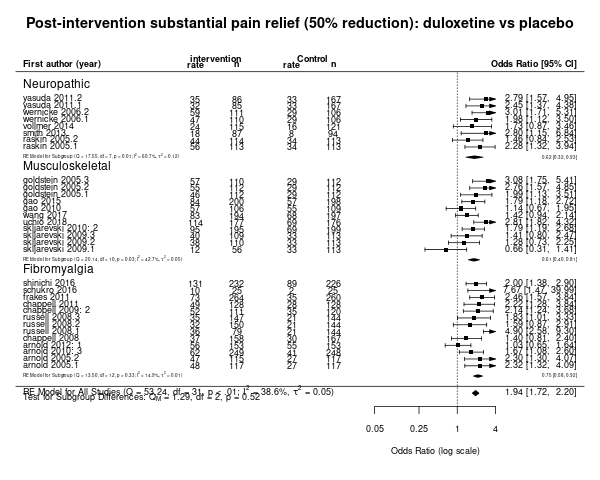
\includegraphics[width=0.5\linewidth,height=0.35\textheight]{img/pain_sub-duloxetine-placebo-forest} 
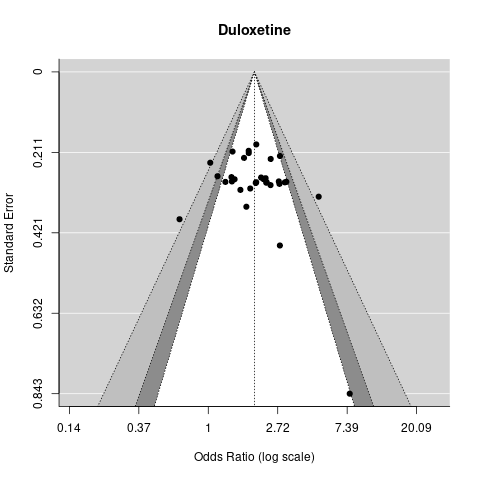
\includegraphics[width=0.5\linewidth,height=0.35\textheight]{img/pain_sub-duloxetine-placebo-funnel} 
\end{knitrout}

\caption{Substantial pain: duloxetine compared with placebo
%\include{"pain\_sub-duloxetine-placebo-rma-caption.txt"}
}
\label{fig:painsub-dulox-plac}
\end{figure}


\subsubsection{Milnacipran}

Meta-analysis of milnacipran was consistent with network meta-analysis estimates. No inconsistency, imprecision, or publication bias detected, however, one third of studies included were high risk of bias. Heterogeneity was not explained by risk of bias or duration of study.


\section{Pain intensity (change scores)}


Pain intensity was reported in 46 studies (3 crossover, 43 parallel) evaluating 46 interventions in trials comprising 14,887 total participants. Studies ran from 5 to 52 weeks, with median length 12 weeks. In the trials reporting placebo, most compared interventions with placebo; with exceptions being two trials comparing duloxetine and pregabalin, and 5 other trials with unqiue comparators. See Summary of findings Table \ref{tab:painint} for the geometry of this network.

\soffignew
{painint}
{img/pain_int-change_score-net.png}
{img/pain_int-change_score-pico.png}
{img/pain_int-change_score-sof.png}
{Pain intensity (change score measures)}

\textbf{Interventions} (number of studies): Placebo (39); duloxetine (27); milnacipran (6); amitriptyline (3); citalopram (2); desipramine (2); paroxetine (2); pregabalin (2); abt-894 (1); cbt (1); cbt and milnacipran (1); desipramine + lidocaine (1); desvenlafaxine (1); esreboxetine (1); fluoxetine (1); gabapentin (1); imipramine (1); lidocaine (1); mirtazapine (1); nortriptyline (1); psychotherapy (1); usual treatment (1).

\subsection{Meta-analyses}


\subsubsection{Duloxetine}

No significant imprecision or inconsistency was detected in duloxetine results. Publication bias was not detected, however there is serious risk of bias in these observations. Heterogeneity was not explained by condition, dose, or duration of studies. No significant inconsistency or imprecision was detected; see, for example, Figure \ref{fig:pain_int-cs-condition-milna-plac}.


\begin{figure}
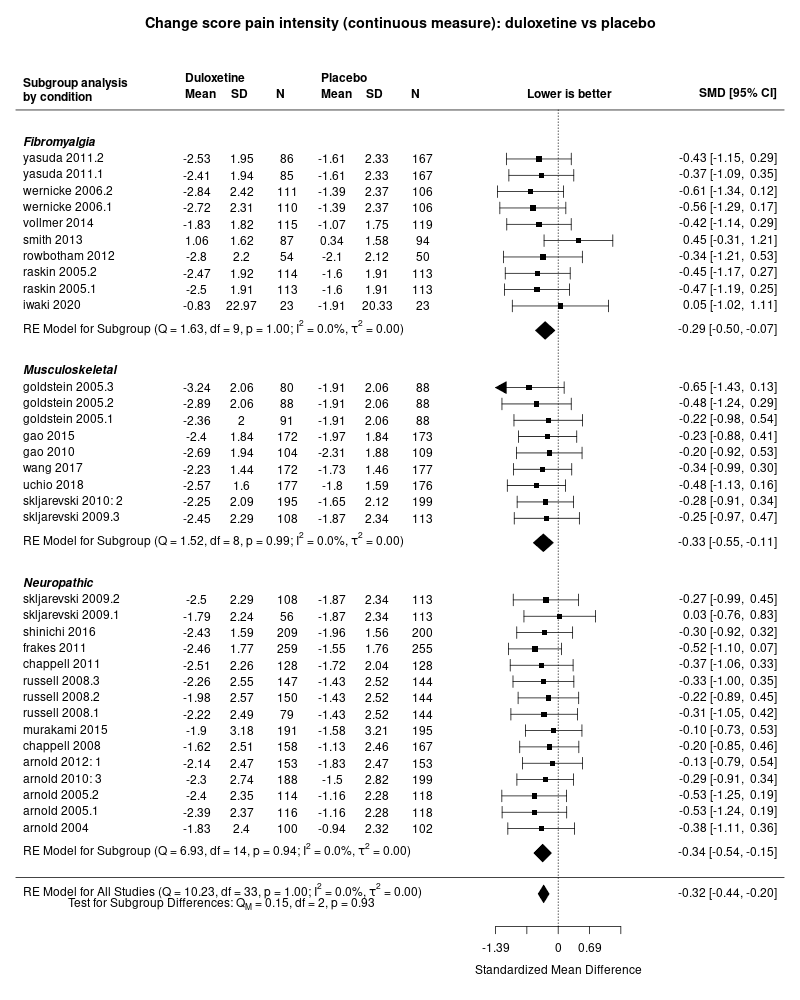
\includegraphics[width=\textwidth]{img/pain_int-change_score-condition-duloxetine-placebo-forest.png}
\caption[Pain intensity by condition: duloxetine]{
Subgroup analysis by condition.
% \input{img/pain_int-change_score-condition-duloxetine-placebo-rma-caption.txt}
}
\label{fig:pain_int-cs-condition-milna-plac}
\end{figure}


\subsubsection{Milnacipran}

No serious inconsistency or imprecision was detected. Risk of bias is serious but publication bias was not detected. Heterogeneity was not explained by condition, dose, risk of bias, or duration of studies.




\section{Pain intensity (post intervention)}


Pain intensity was reported as a post-intervention measure in 80 studies (18 crossover, 62 parallel) evaluating 70 interventions in trials comprising a total of 8016 participants. Studies ran from 2 to 36 weeks, with median length 8 weeks. In post-intervention measures (Summary of findings Table \ref{tab:painintpi}), amitriptyline was compared to benzotropine mesylate in three studies, and amitriptyline against pregablin in two. There were 27 other unique comaparators.

\soffignew
{painintpi}
{img/pain_int-post_int-net.png}
{img/pain_int-post_int-pico.png}
{img/pain_int-post_int-sof.png}
{Pain intensity (post-intervention measures)}

\textbf{Interventions} (number of studies): Placebo (47); amitriptyline (23); duloxetine (13); milnacipran (8); fluoxetine (6); pregabalin (6); benzotropine mesylate (5); gabapentin (4); maprotiline (4); nortriptyline (4); paroxetine (4); cbt (3); escitalopram (3); acupuncture (2); citalopram (2); desipramine (2); melatonin (2); morphine (2); saffron/crocin (2); sertraline (2); venlafaxine (2); active placebo (1); aerobic exercise (1); amitriptyline + fluoxetine (1); amitriptyline + fluphenazine (1); amitriptyline + psychotherapy (1); amitriptyline + riboflavin (vitamin b2) (1); amitriptyline + splint (1); amitriptyline + support (1); benzotropine mesylate + cbt (1); bupropion (1); carbamazepine (1); clomipramine (1); cst (1); cst + sertraline (1); cyclobenzaprine (1); desipramine + cbt (1); diphenhydramine (1); disease management (1); dothiepin (1); education (1); epidural injection (1); epidural injection + amitriptyline (1); esreboxetine (1); fluoxetine + melatonin (1); fluphenazine (1); gabapentin + nortriptyline (1); glycopyrrolate (1); lamotrigine (1); melatonin + amitriptyline (1); mianserin (1); mirtazapine (1); moclobemide (1); morphine + nortriptyline (1); neurofeedback (1); nortriptyline + cbt (1); nortriptyline + disease management (1); nortriptyline + morphine (1); physical therapy (1); pirlindole (1); pregabalin + duloxetine (1); psychotherapy (1); reboxetine (1); riboflavin (vitamin b2) (1); support (1); tens (1); trazodone (1); trazodone + gabapentin (1); trimipramine (1); waitlist (1); zimeldine (1).

Subgroup analysis by dose was not possible with these data.


\subsection{Meta-analyses}

\subsubsection{Duloxetine}

No significant imprecision or inconsistency was detected in duloxetine results. Publication bias was not detected, however there is serious risk of bias in these observations. Heterogeneity of observations for duloxetine was not explained by condition, dose, risk of bias, or duration of study (for example, ).

\subsubsection{Milnacipran}

No serious inconsistency or imprecision was detected. Risk of bias is serious but publication bias was not detected. Heterogeneity of observations for milnacipran was not explained by condition, dose, or duration of study .

\subsubsection{Amitriptyline}

No imprecision, inconsistency, or publication bias was detected, however these observations have serious risk of bias. Heterogeneity of observations for amitriptyline was not explained by condition, risk of bias, or duration of study.



\section{Mood (Change score results)}

37 parllel-design studies reported mood as change-score measures evaluating 18 interventions over a population of 12,697 participants. Studies ran from 6 to 28 weeks, with median length 12 weeks. Three studies did not include placebo trials, using cognitive behavioural therapy, pregabalin, and psychotherapy as comparators with antidepressants. Summary of findings Table \ref{tab:moodcs} shows the network meta-analysis estimates for mood outcomes measured as change scores. These studies ran from 6 to 28 weeks, with median length 12 weeks.

\soffignew
{moodcs}
{img/mood-change_score-net.png}
{img/mood-change_score-pico.png}
{img/mood-change_score-sof.png}
{Mood (change-score measures)}


\textbf{Interventions} (number of studies): Placebo (33); duloxetine (26); milnacipran (4); citalopram (2); pregabalin (2); abt-894 (1); cbt (1); cbt and milnacipran (1); desipramine (1); desipramine + lidocaine (1); esreboxetine (1); fluoxetine (1); imipramine (1); lidocaine (1); mirtazapine (1); nortriptyline (1); paroxetine (1); psychotherapy (1); usual treatment (1).

Conditions: fibromyalgia; musculoskeletal; neuropathic; gastrointestinal; vulvodynia.

Summary of findings (Table \ref{tab:moodcs}) shows 26 studies evaluated duloxetine, 4 studies evaluatede milnacipran, and all other interventions were evalatuated in 1 or 2 studies.

\subsection{Meta-analyses}

\subsubsection{Duloxetine}

Heterogeneity in mood measured as change scores was not explained by condition, dose, duration of study, or risk of bias.

\subsubsection{Milnacipran}

Heterogeneity was not explained by dose.

\subsubsection{Amitriptyline}


\section{Mood (Post intervention results)}

47 studies (9 crossover, 38 parallel) reported mood as post-intervention measures. These studies evaluated 50 interventions over a population of 3804; i.e., this is a network (Summary of findings Table \ref{tab:moodpi}) of several small trial. For post-intervention measures, several other comparators were considered in the literature, notably amitriptyline (7 studies), citalopram (2 studies), fluoxetine (2 studies), and acupuncture (2 studies). Most comparators were either combined or unique, with trials included in only one study. Studies ran from 2 to 34 weeks, with median length 8 weeks.

\soffignew
{moodpi}
{img/mood-post_int-net.png}
{img/mood-post_int-pico.png}
{img/mood-post_int-sof.png}
{Mood (post-intervention measures)}

\textbf{Interventions} (number of studies): Placebo (27); amitriptyline (10); duloxetine (8); benzotropine mesylate (4); fluoxetine (4); pregabalin (4); venlafaxine (4); escitalopram (3); milnacipran (3); nortriptyline (3); paroxetine (3); acupuncture (2); cbt (2); citalopram (2); morphine (2); saffron/crocin (2); aerobic exercise (1); amitriptyline + fluoxetine (1); amitriptyline + fluphenazine (1); amitriptyline + riboflavin (vitamin b2) (1); amitriptyline + splint (1); carbamazepine (1); clomipramine (1); cst (1); cst + sertraline (1); cyclobenzaprine (1); disease management (1); dothiepin (1); fluoxetine + melatonin (1); fluphenazine (1); gabapentin (1); gabapentin + nortriptyline (1); glycopyrrolate (1); maprotiline (1); melatonin (1); mirtazapine (1); moclobemide (1); morphine + nortriptyline (1); neurofeedback (1); nortriptyline + cbt (1); nortriptyline + disease management (1); nortriptyline + morphine (1); pirlindole (1); pregabalin + duloxetine (1); reboxetine (1); riboflavin (vitamin b2) (1); sertraline (1); tens (1); trazodone (1); trimipramine (1); waitlist (1).

Conditions: musculoskeletal; primary; neuropathic; fibromyalgia; atypical facial pain; non-cardiac chest pain; burning mouth syndrome; phantom/residual limb pain; unspecified.

In Summary of Findings Table \ref{tab:moodpi}, there are 10 studies that evaluate amitriptyline and 8 that evaluate duloxetine. Of the 50 interventions evaluated, most are included in 3 studies or fewer.

\subsection{Meta-analyses}

\subsubsection{Duloxetine}

Heterogeneity was not explained by dose. Possibly some heterogeneity is explained by duration of study (Figure \ref{fig:moodpi-duration-dulox-plac}).

\begin{figure}
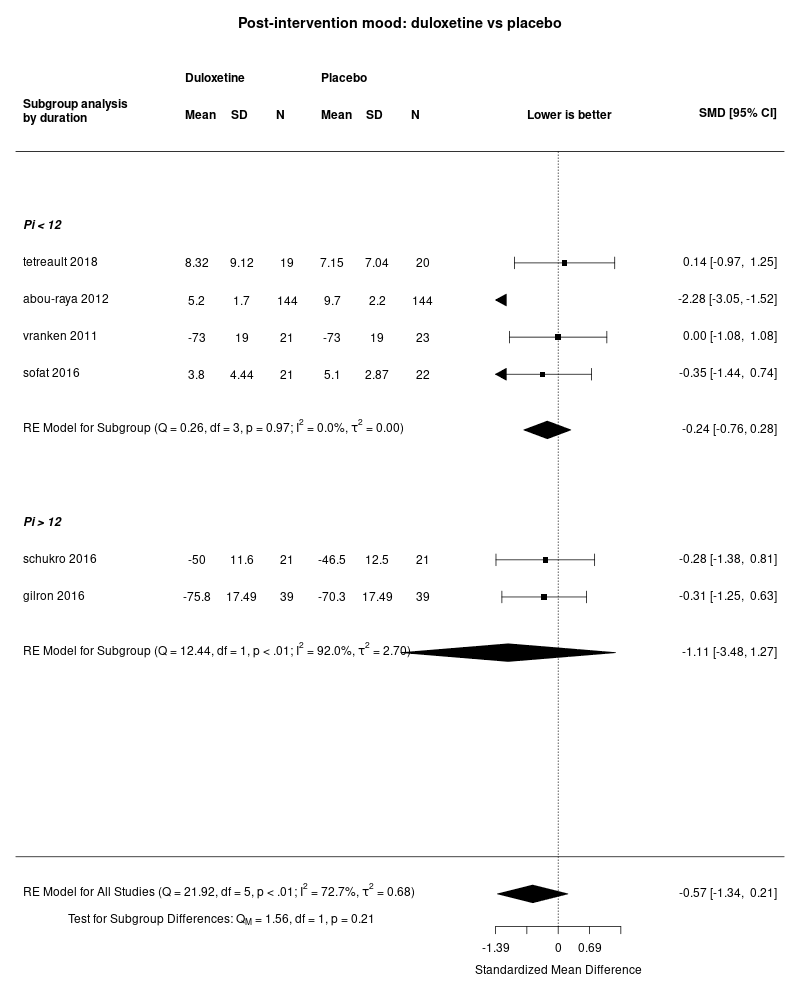
\includegraphics[width=\textwidth]{img/mood-post_int-duration-duloxetine-placebo-forest.png}
\caption[Mood by duration, duloxetine]{Subgroup analysis by duration of study.}
\label{fig:moodpi-duration-dulox-plac}
\end{figure}

\section{Mood}

Mood was reported in 84 studies with 37 parallel-design studies reporting change score (CS) measures and 47 studies reporting post intervention (PI) measures (9 crossover, 38 parallel design). These trials include 16501 participants (CS 12,697, PI 3804) and comparing interventions (CS 18, PI 50) for adults with chronic pain. The direct evidence networks for the two measurement groups are shown in Summary of findings Tables \ref{tab:moodcs} and \ref{tab:moodpi}.

\section{Adverse events}


Adverse events were reported in 90 studies (15 crossover, 75 parallel design) including 21,718 participants and comparing 46 interventions for adults with chronic pain. The length of trials ranged from 2 to 34 weeks, with a median length of 10 weeks. Summary of findings (Table \ref{tab:adverse}) shows a disconnected network. In addition to placebo, three studies compared duloxetine to pregabline, 2 compared amitriptyline to benzotropine mesylate, and 2 further studies compared amitriptyline to gabapentin. There were 16 comparators unique to single trials.

\soffignew
{adverse}
{img/adverse-post_int-net.png}
{img/adverse-pico.png}
{img/adverse-sof.png}
{Adverse events}

\textbf{Interventions} (number of studies): Placebo (67); duloxetine (29); amitriptyline (18); milnacipran (15); venlafaxine (6); gabapentin (5); pregabalin (5); benzotropine mesylate (4); imipramine (4); carbamazepine (3); nortriptyline (3); paroxetine (3); cbt (2); desipramine (2); desvenlafaxine (2); esreboxetine (2); mirtazapine (2); abt-894 (1); acetaminophen (1); active placebo (1); benzotropine mesylate + cbt (1); cbt and milnacipran (1); citalopram (1); clonidine (1); cst (1); cst + sertraline (1); cyclobenzaprine (1); desipramine + cbt (1); disease management (1); dothiepin (1); escitalopram (1); fluvoxamine (1); lamotrigine (1); lorazepam (1); maprotiline (1); melatonin (1); melatonin + amitriptyline (1); moclobemide (1); morphine (1); morphine + nortriptyline (1); nortriptyline + cbt (1); nortriptyline + disease management (1); pirlindole (1); pregabalin + imipramine (1); reboxetine (1); sertraline (1); trazodone + gabapentin (1).




\subsection{Meta-analyses}

\subsubsection{Duloxetine}

The direct evidence for duloxetine compared with placebo was consistent with the network meta-analysis estimates, however publication bias (Figure \ref{fig:adverse-dulox-plac}) is strongly suspected, also implied by the comparison of duloxetine and pregabalin (Figure \ref{fig:adverse-dulox-pregab}). Heterogeneity in duloxetine observations were not explained by condition, dose, or duration of studies.


\begin{figure}
\begin{knitrout}
\definecolor{shadecolor}{rgb}{0.969, 0.969, 0.969}\color{fgcolor}
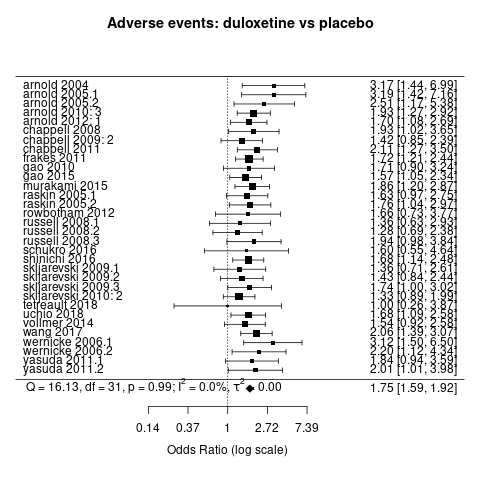
\includegraphics[width=0.5\linewidth,height=0.35\textheight]{img/adverse-duloxetine-placebo-forest} 
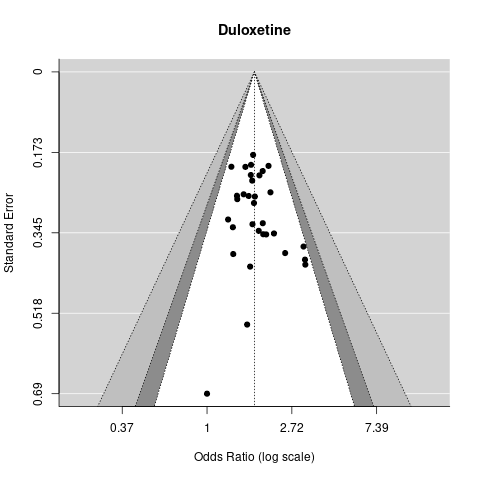
\includegraphics[width=0.5\linewidth,height=0.35\textheight]{img/adverse-duloxetine-placebo-funnel} 
\end{knitrout}

\caption[Adverse: duloxetine vs pregabalin]{\input{img/adverse-duloxetine-placebo-rma-caption.txt}}
\label{fig:adverse-dulox-plac}
\end{figure}



\begin{figure}
\begin{knitrout}
\definecolor{shadecolor}{rgb}{0.969, 0.969, 0.969}\color{fgcolor}
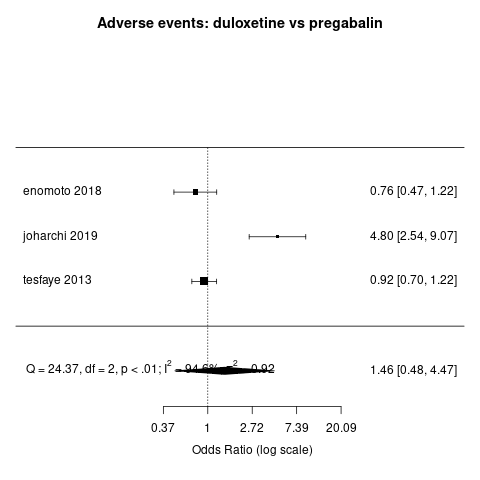
\includegraphics[width=0.5\linewidth,height=0.35\textheight]{img/adverse-duloxetine-pregabalin-forest} 
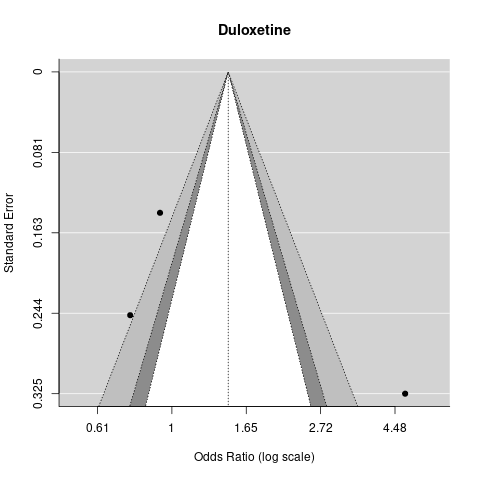
\includegraphics[width=0.5\linewidth,height=0.35\textheight]{img/adverse-duloxetine-pregabalin-funnel} 
\end{knitrout}

\caption[Adverse: duloxetine vs pregabalin]{\input{img/adverse-duloxetine-pregabalin-rma-caption.txt}}
\label{fig:adverse-dulox-pregab}
\end{figure}





\subsubsection{Milnacipran}

Studies evaluating milnacipran compared with placebo showed some inconsistency and publication bias (Figure \ref{fig:adverse-milna}).

\begin{figure}

\begin{knitrout}
\definecolor{shadecolor}{rgb}{0.969, 0.969, 0.969}\color{fgcolor}
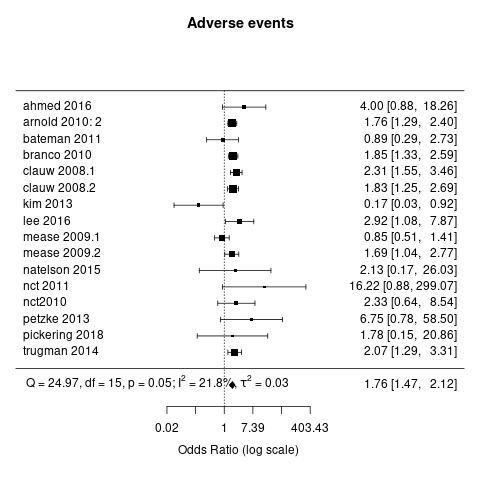
\includegraphics[width=0.5\linewidth,height=0.35\textheight]{img/adverse-milnacipran- - -forest} 
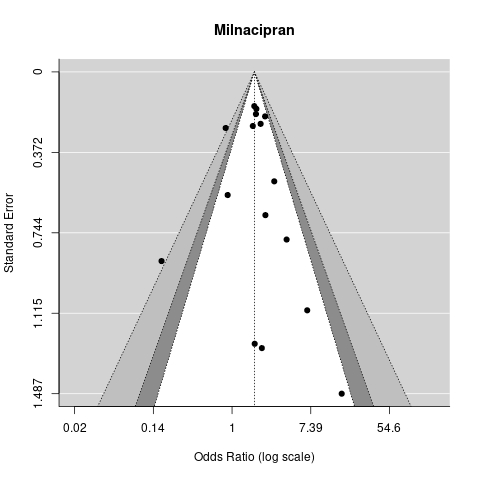
\includegraphics[width=0.5\linewidth,height=0.35\textheight]{img/adverse-milnacipran- - -funnel} 
\end{knitrout}

\caption[Adverse events: milnacipran]{Outcome: adverse events. Measure: post-intervention. Intervention: milnacipran. Participants: 5455. Direction of improvement: lower. Meta-analysis results: Q = 24.97; df = 15; p = 0.05; $I^2$ = 21.85 per cent; $\tau^2$ = 0.03. Regression test for funnel plot asymmetry was significant: 0.51 (CI 0.2 to 0.83) with p = 0.69 and z = 0.4.}
\label{fig:adverse-milna}
\end{figure}


Heterogeneity observed in adverse events for milnacipran compared to placebo showed some difference (Figure \ref{fig:adverse-condition-milna-plac}) between fibromyalgia and musculoskeletal patients. Heterogeneity of milnacipran observations was not explained by duration of studies.

\begin{figure}

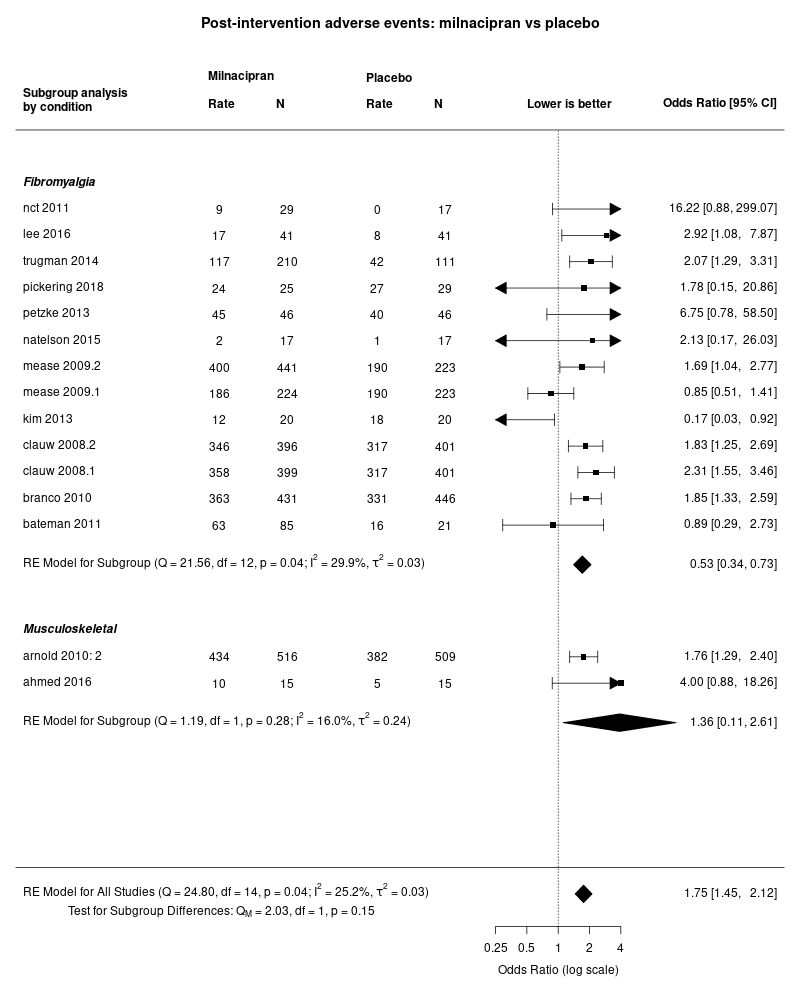
\includegraphics[width=\textwidth]{img/adverse-condition-milnacipran-placebo-forest.png}
\caption[Adverse by condition: milnacipran]{
Subgroup analysis by condition. \input{img/adverse-condition-milnacipran-placebo-rma-caption.txt}
}
\label{fig:adverse-condition-milna-plac}
\end{figure}

Some heterogeneity is also explained by dose, where there is inconsistency and significant imprecision between groups (Figure \ref{fig:adverse-dose-milna-plac}).


\begin{figure}

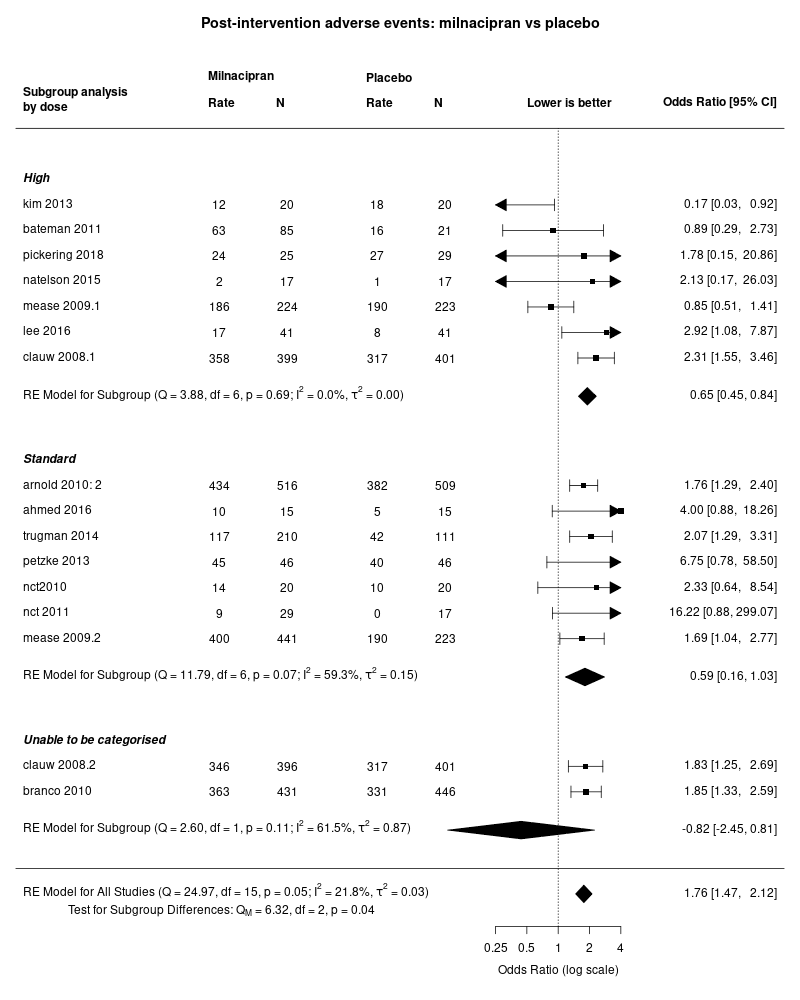
\includegraphics[width=\textwidth]{img/adverse-dose-milnacipran-placebo-forest.png}
\caption[adverse by dose: milnacipran]{
Subgroup analysis by dose. \input{img/adverse-dose-milnacipran-placebo-rma-caption.txt}
}
\label{fig:adverse-dose-milna-plac}
\end{figure}

\subsubsection{Amitriptyline}

Amitriptyline results were inconsistent, with serious risk of bias, and there is some indication of publication bias (Figure \ref{fig:adverse-amitrip}).

\begin{figure}

\begin{knitrout}
\definecolor{shadecolor}{rgb}{0.969, 0.969, 0.969}\color{fgcolor}
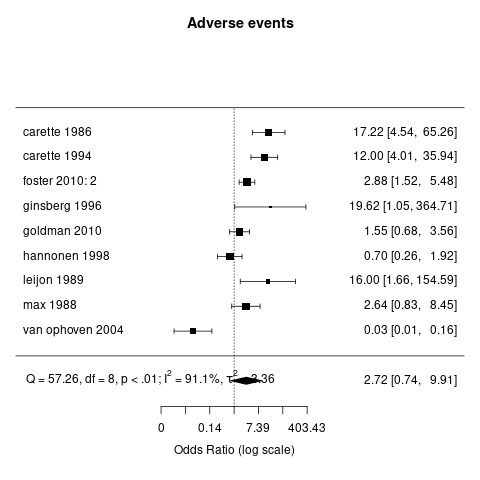
\includegraphics[width=0.5\linewidth,height=0.35\textheight]{img/adverse-amitriptyline- - -forest} 
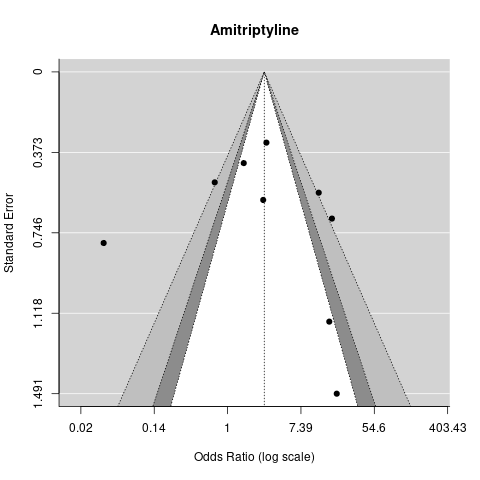
\includegraphics[width=0.5\linewidth,height=0.35\textheight]{img/adverse-amitriptyline- - -funnel} 
\end{knitrout}

\caption[Adverse events: amitriptyline]{Outcome: adverse events. Measure: post-intervention. Intervention: amitriptyline. Participants: 915. Direction of improvement: lower. Meta-analysis results: Q = 57.26; df = 8; p $<$ .01; $I^2$ = 91.1 per cent; $\tau^2$ = 3.36. Regression test for funnel plot asymmetry was not significant: -0.13 (CI -3.25 to 2.99) with p = 0.43 and z = 0.79.}
\label{fig:adverse-amitrip}
\end{figure}


Some heterogeneity is possibly explained by differences between conditions (Figure \ref{fig:adverse-condition-amitr-plac})

\begin{figure}

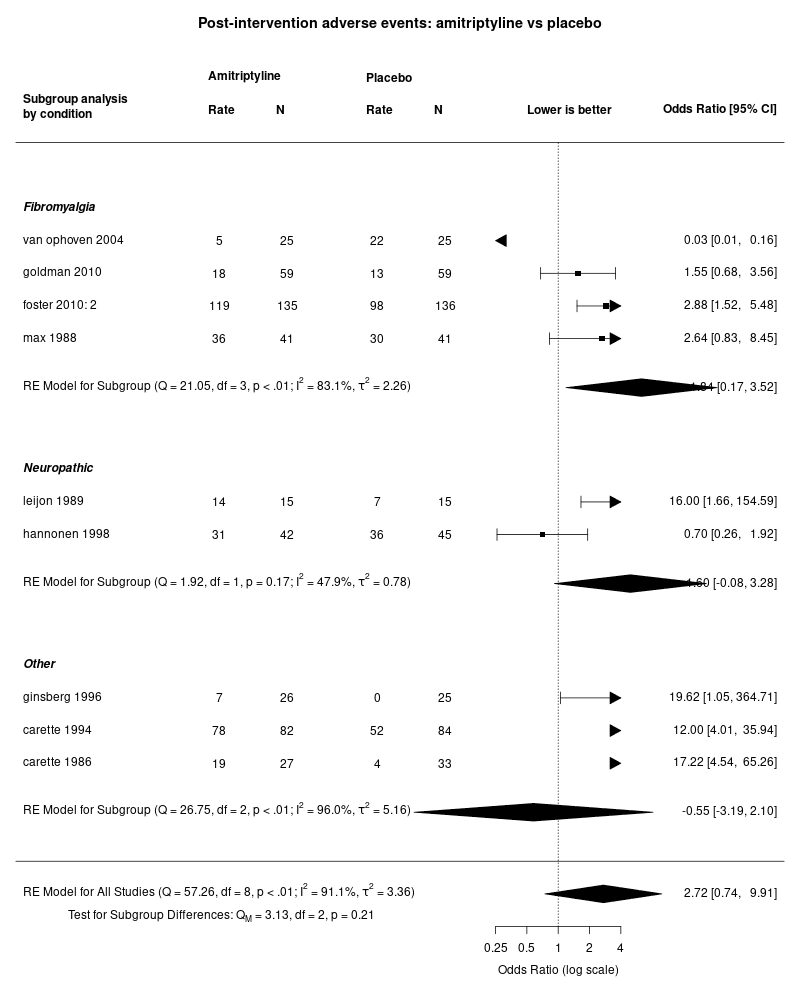
\includegraphics[width=\textwidth]{img/adverse-condition-amitriptyline-placebo-forest.png}
\caption[Adverse by condition: amitriptyline]{
Subgroup analysis by condition. \input{img/adverse-condition-amitriptyline-placebo-rma-caption.txt}
}
\label{fig:adverse-condition-amitr-plac}
\end{figure}

There was significant heteregenity and imprecision between subgroups by duration of study for amitriptyline (Figure \ref{fig:adverse-duration-amitr-plac}).


\begin{figure}

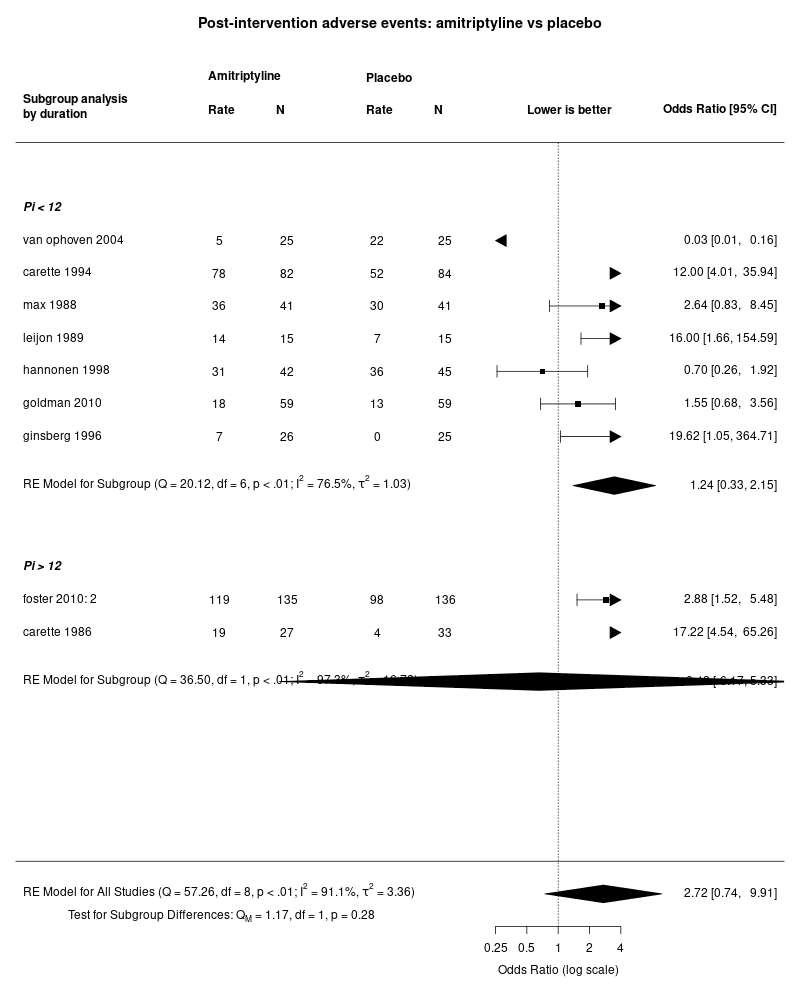
\includegraphics[width=\textwidth]{img/adverse-duration-amitriptyline-placebo-forest.png}
\caption[Adverse by duration: amitriptyline]{
Subgroup analysis by duration. \input{img/adverse-duration-amitriptyline-placebo-rma-caption.txt}
}
\label{fig:adverse-duration-amitr-plac}
\end{figure}

\chapter{Secondary outcomes}


\section{Serious adverse events (SAE)}

SAE were reported in 60 studies (8 crossover, 52 parallel) evaluating 30 interventions including 16,138 participants with one of seven pain conditions. The studies ranged from  2 to 34 weeks with most studies lasting 12 weeks. Summary of findings \ref{tab:serious} shows the direct evidence network for SAE wherein there were many more participants in milnacipran and duloxetine trials than any other intervention. Aside from 2 studies comparing duloxetine to pregablin, all other interventions evaluated by more than one study compared intervention  to placebo. There are several single-study comparisons between other combinations.

\soffignew
{serious}
{img/serious_adverse-post_int-net.png}
{img/serious_adverse-pico.png}
{img/serious_adverse-sof.png}
{SAE (Serious adverse events)}

\textbf{Interventions} (number of studies): Placebo (51); duloxetine (21); milnacipran (14); amitriptyline (6); paroxetine (4); mirtazapine (3); pregabalin (3); carbamazepine (2); citalopram (2); desvenlafaxine (2); nortriptyline (2); venlafaxine (2); benzotropine mesylate (1); benzotropine mesylate + cbt (1); bupropion (1); cbt (1); cst (1); cst + sertraline (1); desipramine (1); desipramine + cbt (1); disease management (1); esreboxetine (1); fluvoxamine (1); gabapentin (1); gabapentin + nortriptyline (1); imipramine (1); nabilone (1); nortriptyline + cbt (1); nortriptyline + disease management (1); reboxetine (1); sertraline (1).


\subsection{Meta-analyses}


There were only enough data to undertake subgroup analysis by condition for duloxetine.

\subsubsection{Duloxetine}

Duloxetine observations did not display inconsistency or imprecision, however there is serious risk of bias. Heterogeneity in duloxetine compared to placebo observations was not explained by condition, risk of bias, or duration of study.

\subsubsection{Milnacipran}

Heterogeneity of milnacipran compared to placebo was not explained by duration of study or risk of bias. Imprecision is present in these observations(Figure \ref{fig:sae-milna-plac}). There is no strong indication of risk of bias, however these observation have very serious risk of bias.

\begin{figure}


\begin{knitrout}
\definecolor{shadecolor}{rgb}{0.969, 0.969, 0.969}\color{fgcolor}
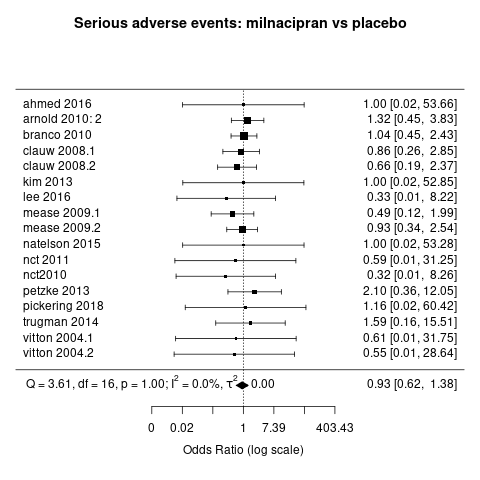
\includegraphics[width=0.5\linewidth,height=0.35\textheight]{img/serious_adverse-milnacipran-placebo-forest} 
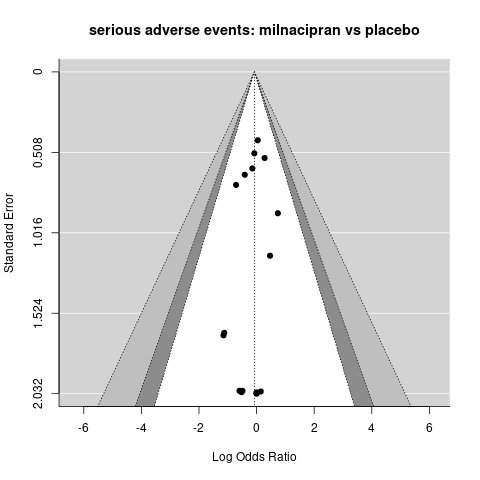
\includegraphics[width=0.5\linewidth,height=0.35\textheight]{img/serious_adverse-milnacipran-placebo-funnel} 
\end{knitrout}

\caption[SAE, amitriptyline]{\input{
img/serious_adverse-amitriptyline-placebo-rma-caption.txt}}
\label{fig:sae-milna-plac}
\end{figure}


\subsubsection{Amitritptyline}

There is significant imprecision in these observations (Figure \ref{fig:sae-ami-plac}); serious risk of bias is suspected.

\begin{figure}
\centering
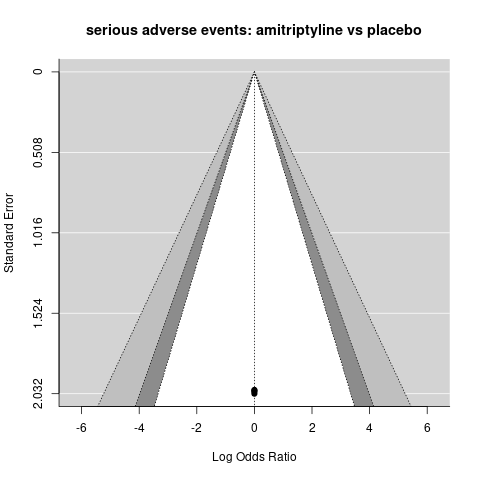
\includegraphics[width=0.5\textwidth]{
img/serious_adverse-amitriptyline-placebo-funnel.png}
\caption[SAE, amiptriptyline]{\input{
img/serious_adverse-amitriptyline-placebo-rma-caption.txt}}
\label{fig:sae-ami-plac}
\end{figure}


\section{Dropout due to adverse events}

Dropout due to adverse events was widely reported, in 110 studies (20 crossover, 90 parallel), evaluating 59 interventions over a population of 23,950. The studies ran from 2 to 34 weeks, with a median length of 10 weeks. The complexity of the network geometry (Summary of findings \ref{tab:dropout}) is driven by the number of interventions and comparators. However, the majority of trials were in duloxetine, amitriptyline, and milnacipran. The population were primarily fibromyalgia, neuropathic, and musculoskeleetal pain patients. Pregabalin was used as a comparator against duloxetine in three studies, and benotropine mesylate was compared again amitriptyline in two studies. The other comparators were unique to single trials.

\soffignew
{dropout}
{img/adverse_dropout- - -post_int-net.png}
{img/adverse_dropout-pico.png}
{img/adverse_dropout-sof.png}
{Dropout due to adverse events}

\textbf{Interventions} (number of studies): Placebo (82); Duloxetine (32); Amitriptyline (25); Milnacipran (12); Pregabalin (8); Gabapentin (6); Venlafaxine (6); Nortriptyline (5); Paroxetine (5); Benzotropine mesylate (4); Fluoxetine (4); Carbamazepine (3); Desipramine (3); Imipramine (3); Mirtazapine (3); Cbt (2); Citalopram (2); Escitalopram (2); Esreboxetine (2); Maprotiline (2); Morphine (2); Sertraline (2); Trazodone (2); Acetaminophen (1); Amitriptyline + fluoxetine (1); Amitriptyline + fluphenazine (1); Amitriptyline + naproxen (1); Amitriptyline + riboflavin (vitamin b2) (1); Benzotropine mesylate + cbt (1); Bupropion (1); Clomipramine (1); Cst (1); Cst + sertraline (1); Cyclobenzaprine (1); Desipramine + cbt (1); Desipramine + lidocaine (1); Desvenlafaxine (1); Diphenhydramine (1); Doxepin (1); Education (1); Fluphenazine (1); Gabapentin + nortriptyline (1); Glycopyrrolate (1); Lidocaine (1); Lorazepam (1); Melatonin (1); Melatonin + amitriptyline (1); Moclobemide (1); Morphine + nortriptyline (1); Naproxen (1); Nortriptyline + morphine (1); Physical therapy (1); Pirlindole (1); Pregabalin + duloxetine (1); Pregabalin + imipramine (1); Reboxetine (1); Riboflavin (vitamin b2) (1); Trazodone + gabapentin (1); Trimipramine (1); Zimeldine (1).

\subsection{Meta-analysis results}

\subsubsection{Duloxetine}

When all trials are considered, i.e., across all doses,  conditions, and other subgroups, meta-analytic results for duloxetine are consistent with the estimates of the network analysis. 0.4 of studies were ranked as high risk of bias. Some heterogeneity is explained by difference between pain condition groups (Figure \ref{fig:dropout-condition-dulox-plac}), where neuropathic patients are morelikely to drop out of the study due to adverse events than fibromyalgia patients.

\begin{figure}
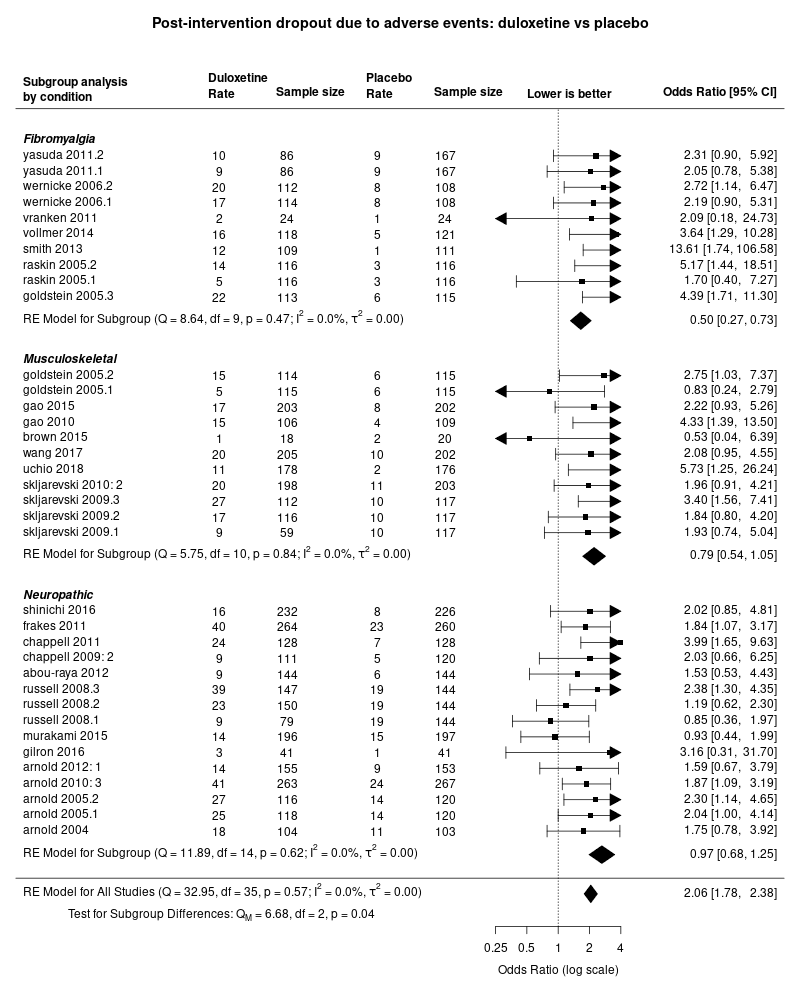
\includegraphics[width = \textwidth]{img/adverse_dropout-condition-duloxetine-placebo-forest.png}
\caption[Dropout by condition, duloxetine]{
Subgroup analysis by condition.
\input{img/adverse_dropout-condition-duloxetine-placebo-rma-caption.txt}
}
\label{fig:dropout-condition-dulox-plac}
\end{figure}

There was not as much difference between different dose groups (Figure \ref{fig:dropout-dose-dulox-plac}), but the higher the dosage, the more likely the participant was to drop out to adverse events. No heterogeneity was explained by risk of bias or duration of study.

\begin{figure}
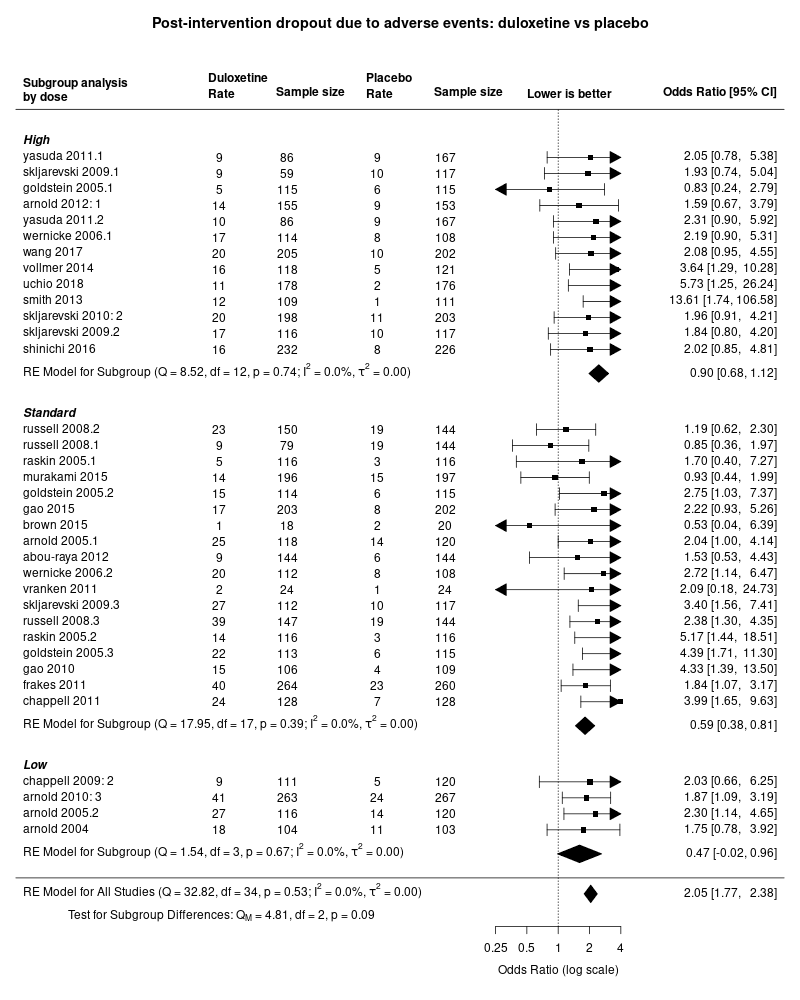
\includegraphics[width = \textwidth]{img/adverse_dropout-dose-duloxetine-placebo-forest.png}
\caption[Dropout by dose, duloxetine]{
Subgroup analysis by dose.
\input{img/adverse_dropout-dose-duloxetine-placebo-rma-caption.txt}
}
\label{fig:dropout-dose-dulox-plac}
\end{figure}



\subsubsection{Amitriptyline}

As with duloxetine, above, amitriptyline trials were consistent within themselves, and with the network meta-anlaysis estimates. 0.5 of studies were raked as high risk of bias. Subgroup analysis by duration of study did not explain any heterogeneity observed.

\subsubsection{Milnacipran}

Meta-analysis results for milnacipran were consistent with network meta-analysis findings. 0.8 of studies were high risk of bias, and publication bias was also detected. Some heterogeneity explained by duration of study (Figure \ref{fig:dropout-duration-milna-plac}), with participants in trials lasting more than 12 weeks signficantly more likely to drop out due to adverse events.

\begin{figure}
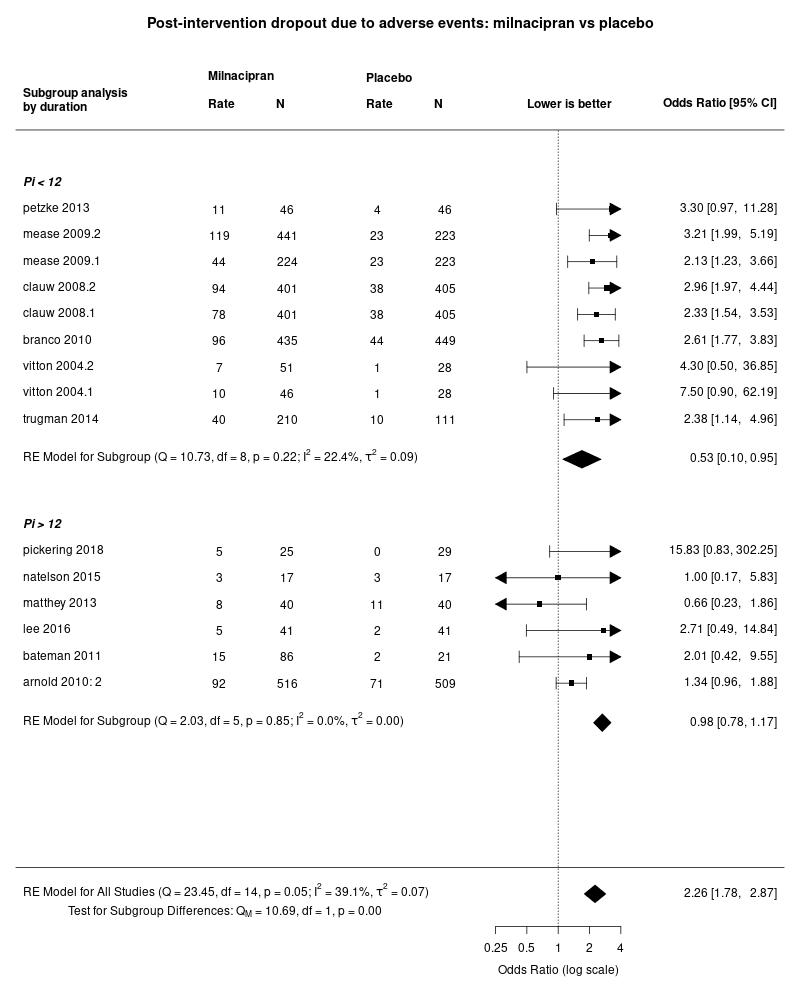
\includegraphics[width = \textwidth]{img/adverse_dropout-duration-milnacipran-placebo-forest.png}
\caption[Dropout by duration, milnacipran]{
Subgroup analysis by duration.
}
\label{fig:dropout-duration-milna-plac}
\end{figure}



\section{Moderate pain relief (30 per cent reduction)}

Moderate pain was reported in 41 studies (5 crossover, 36 parallel) evaluating 21 interventions over a total of 14,240 participants. The studies ran from 4 to 28 weeks, with a median length of 12 weeks. The network geometry shown in Summary of findings Table \ref{tab:painmod}  is disconnected, with unique comparators within single trials. Comparators, other than placebo, were pregablin, amitriptyline, cognitive behavioural therapy, nortriptyline, and morphine. Pregablin was used as comparator in two studies, and the rest in single trials.

\soffignew
{painmod}
{img/pain_mod-post_int-net.png}
{img/pain_mod-pico.png}
{img/pain_mod-sof.png}
{Moderate pain relief (30\% reduction)}

\textbf{Interventions}: Placebo (32); Duloxetine (25); Milnacipran (7); Pregabalin (4); Amitriptyline (2); Esreboxetine (2); Mirtazapine (2); Nortriptyline (2); Benzotropine mesylate (1); Benzotropine mesylate + cbt (1); Carbamazepine (1); Cbt (1); Cbt and milnacipran (1); Desipramine (1); Desipramine + cbt (1); Diphenhydramine (1); Gabapentin (1); Imipramine (1); Morphine (1); Nortriptyline + morphine (1); Pregabalin + imipramine (1); Venlafaxine (1).

\subsubsection{Summary of head to head comparisons}

Head-to-head comparison by condition was only posssible for duloxetine. There was no difference for all possible comparisons (duloxetine and milnacipran) by duration of study (less than 12 weeks or greater).

\subsection{Meta-analyses}

\subsubsection{Duloxetine}

Meta-analysis comparing duloxetine to placebo produces the same results as for substantial pain (see Figure \ref{fig:painsub-dulox-plac}); i.e., consistent, precise, in keeping with the network meta-analysis results, but some indication of publication bias (not significant). Subgroup analysis (Figure \ref{fig:painmod-condition-dulox}) by condition showed some difference between musculoskeletal patients and other pain conditions.

\begin{figure}
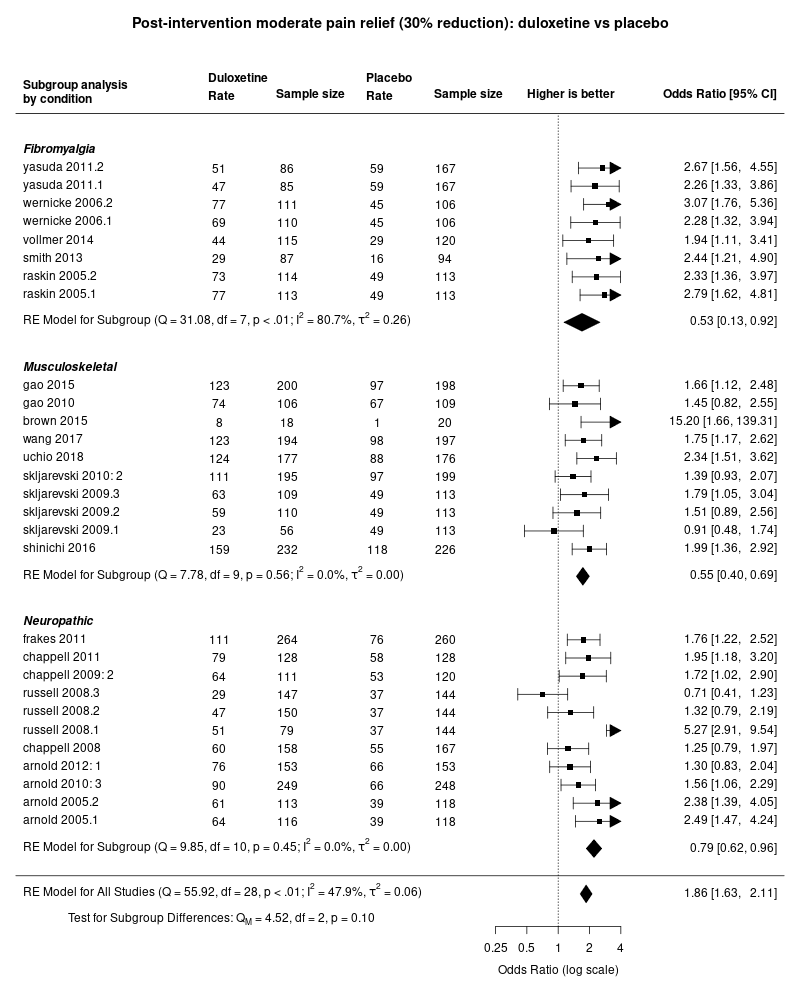
\includegraphics[width = \textwidth]{img/pain_mod-condition-duloxetine-placebo-forest.png}
\caption[Moderate pain relief by condition, duloxetine]{Subgroup analysis by condition.
\input{img/pain_mod-condition-duloxetine-placebo-rma-caption.txt}
}
\label{fig:painmod-condition-dulox}
\end{figure}

Heterogeneity of duloxetine (Figure \ref{fig:painmod-dose-dulox}) is partly explained by dose, where low dose does not show an effect. There was not a significant difference between high and low risk of bias studies comparing duloxetine with placebo. Similarly, no difference by duration of study.

\begin{figure}
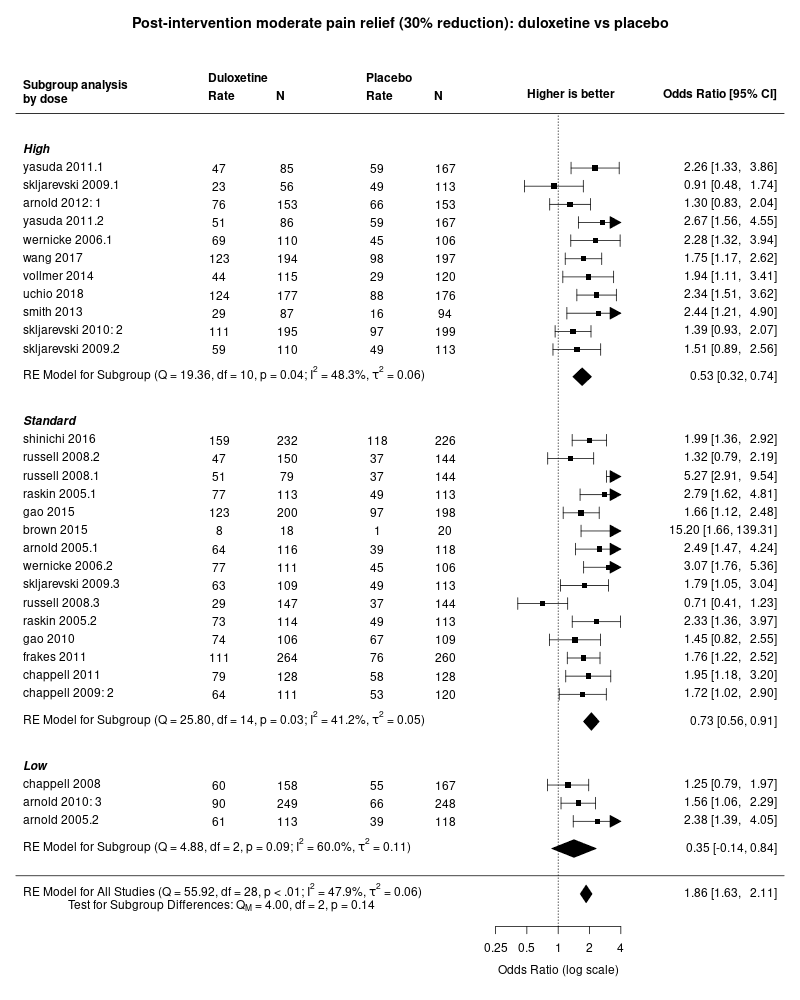
\includegraphics[width = \textwidth]{img/pain_mod-dose-duloxetine-placebo-forest.png}
\caption[Moderate pain relief by dose, duloxetine]{Subgroup analysis by dose.
\input{img/pain_mod-dose-duloxetine-placebo-rma-caption.txt}
}
\label{fig:painmod-dose-dulox}
\end{figure}


\subsubsection{Milnacipran}

No publication bias, inconsistency, or imprecision detected for milnacipran. However, the proportion of studies with high risk of bias is 0.86. All milnacipran trials were in fibromyalgia patients. There was not a significant difference between dosages at high, standard, and dosages unable to be categorised. Similarly, no difference between long and short duration studies.


\section{PGIC (Much or very much improved)}

Patient global impression of change (PGIC) measured as \emph{much or very much improved} was reported in 13 parallel-design studies evaluating 6 interventions, of which only one study did not include a placebo trial, including 7258 participants (4541 intervention, 2717 placebo). Studies ran from 6 to 27 weeks, with a median length of 14 weeks. The direct evidence network in Summary of findings \ref{tab:pgicmuch} shows that aside from one study comparing paroxetine and amitriptyline, all other studies included a placebo trial and only one SNRI intervention.

\soffignew
{pgicmuch}
{img/pgic_much_or_very_much_improved-post_int-net.png}
{img/pgic_much_or_very_much_improved-pico.png}
{img/pgic_much_or_very_much_improved-sof.png}
{PGIC (Much or very much improved)}

\textbf{Interventions} (number of studies): Placebo (12); duloxetine (5); milnacipran (5); amitriptyline (1); desvenlafaxine (1); esreboxetine (1); paroxetine (1).


\subsection{Meta-analyses}

Subgroup analyses were not possible with these data.

\subsubsection{Duloxetine}

In Figure \ref{fig:pgic_much_or_very_much_improved-cs-dulox} we see duloxetine compared to placebo does not display imprecision or inconsistency, however, from visual inspection there is some indication of publication bias. These observations have serious risk of bias.

\begin{figure}

\begin{knitrout}
\definecolor{shadecolor}{rgb}{0.969, 0.969, 0.969}\color{fgcolor}
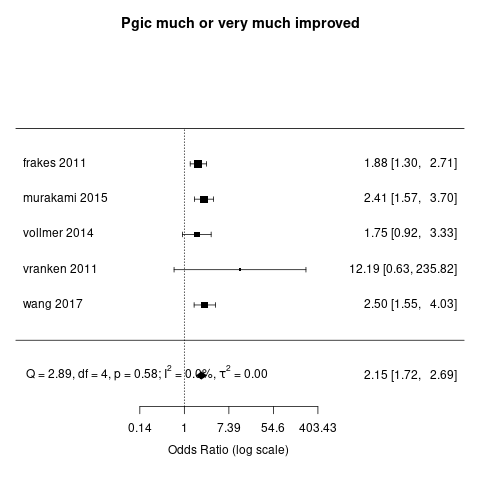
\includegraphics[width=0.5\linewidth,height=0.35\textheight]{img/pgic_much_or_very_much_improved-duloxetine- - -forest} 
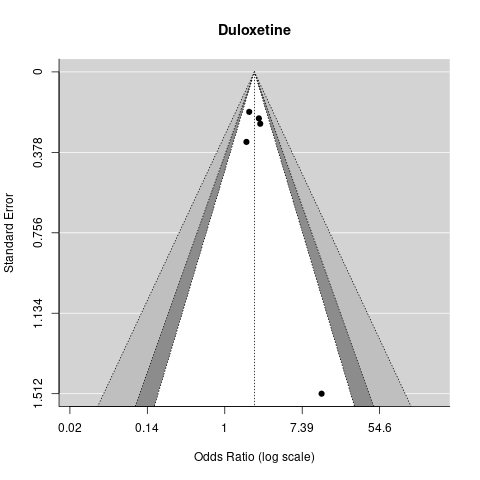
\includegraphics[width=0.5\linewidth,height=0.35\textheight]{img/pgic_much_or_very_much_improved-duloxetine- - -funnel} 
\end{knitrout}

\caption[PGIC (much improved): duloxetine]{
\input{img/pgic_much_or_very_much_improved-duloxetine- - -pw-caption.txt}
}
\label{fig:pgic_much_or_very_much_improved-cs-dulox}
\end{figure}

\subsubsection{Milnacipran}

Milnacipran observations display significant publication bias (Figure \ref{fig:pgic_much_or_very_much_improved-milna}), and are of very serious risk of bias.


\begin{figure}

\begin{knitrout}
\definecolor{shadecolor}{rgb}{0.969, 0.969, 0.969}\color{fgcolor}
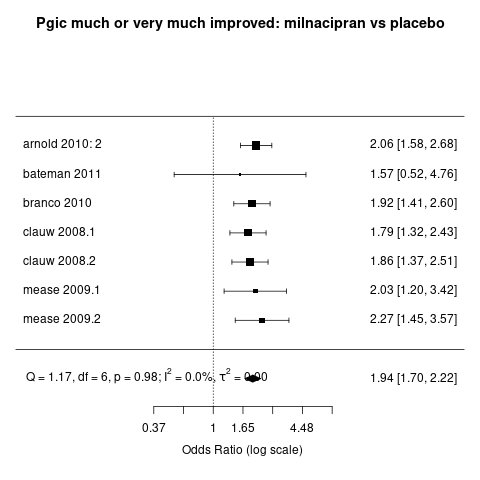
\includegraphics[width=0.5\linewidth,height=0.35\textheight]{img/pgic_much_or_very_much_improved-milnacipran-placebo-forest} 
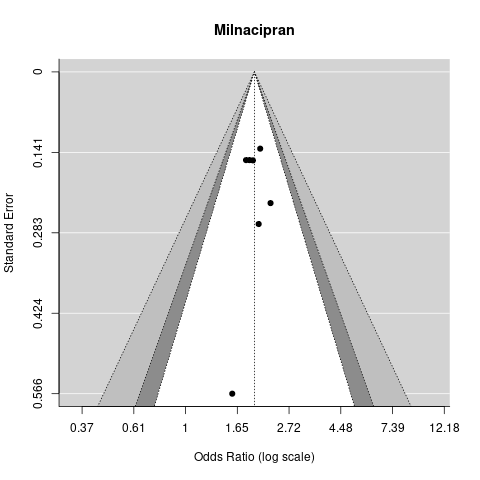
\includegraphics[width=0.5\linewidth,height=0.35\textheight]{img/pgic_much_or_very_much_improved-milnacipran-placebo-funnel} 
\end{knitrout}

\caption[PGIC (much improved): milnacipran]{
\input{img/pgic_much_or_very_much_improved-milnacipran-placebo-rma-caption.txt}
}
\label{fig:pgic_much_or_very_much_improved-milna}
\end{figure}


\section{PGIC (Any improvement)}

Patient global impression of change (PGIC) measured as \emph{any improvement} was reported in 5 studies (2 crossover, 3 parallel) evaluating 5 interventions over trials including 550 participants (365 intervention, 185 placebo). Summary of findings \ref{tab:pgicany} shows a disconnected network, wherein most comparisons are with placebo, the exceptions being one study comparing pregabalin and amitriptyline, and another study comparing carbaqmazepine with amitriptyline. Studies ran from 4 to 13 weeks, with most studies lasting 8 weeks.

\soffignew
{pgicany}
{img/pgic_any_improvement-post_int-net.png}
{img/pgic_any_improvement-pico.png}
{img/pgic_any_improvement-sof.png}
{PGIC (Any improvement)}

\textbf{Interventions} (number of studies): Placebo (4); amitriptyline (2); carbamazepine (1); esreboxetine (1); milnacipran (1); mirtazapine (1); pregabalin (1).

No two comparisons were the same in these trials, so no head-to-head analyses were possible from this dataset.

\section{PGIC (Continuous measures)}

Patient global impression of change (PGIC) was reported as a continuous measure in 5 studies (2 crossover, 3 parallel) evaluating 6 interventions in trials comprising 550 total participants. Studies ran from 4 to 13 weeks with a median length of 8 weeks. The network geometry in Summary of findings Table \ref{tab:pgiccont} shows that all studies bar one compared a single intervention with placebo, with two exceptions for amitriptyline and pregabalin, and a comparison between amitriptyline and carbamezepine.

\soffignew
{pgiccont}
{img/pgic_cont-post_int-net.png}
{img/pgic_cont-post_int-pico.png}
{img/pgic_cont-post_int-sof.png}
{PGIC (post intervention)}

\textbf{Interventions} (number of studies): Duloxetine (22); placebo (20); pregabalin (2); abt-894 (1); desvenlafaxine (1).

It was only possible to run subgroup analyses for duloxetine.

\subsection{Meta-analyses}

\subsubsection{Duloxetine}

Heterogeneity for duloxetine compared with placebo was not explained by condition, dose, duration of study, or risk of bias, when duloxetine was considered under subgroup meta-analyses. Some funnel plot asymmetry was visually detected, but was not significant, suggesting there may be publication bias.


\section{Withdrawal}

Withdrawal was reported in 146 studies (22 crossover, 124 parallel) evaluating 82 interventions in trials comprising 27,288 total participants. Studies ran from 2 to 34 weeks, with most studies lasting 9 weeks. In the trials reporting placebo, most compared interventions with placebo. The geometry of the network (Summary of findings Table \ref{tab:withdrawal}) shows the majority of trials to compare duloxetine, amitriptyline, and milnacipran against placebo. 3 studies compared amitriptyline and benozotropine mesylate, and another 3 studies compared duloxetine and pregabalin; there were 36 other comparators, in addition to placebo, unique to a single trial. The population were primarily fibromyalgia, neuropathic, and musculoskeletal pain patients.

\soffignew
{withdrawal}
{img/withdrawal-post_int-net.png}
{img/withdrawal-pico.png}
{img/withdrawal-sof.png}
{Withdrawal}

\textbf{Interventions} (number of studies): Placebo (104); duloxetine (39); amitriptyline (32); milnacipran (17); pregabalin (9); nortriptyline (7); paroxetine (7); venlafaxine (7); fluoxetine (6); gabapentin (6); benzotropine mesylate (5); cbt (5); citalopram (4); desipramine (4); imipramine (4); carbamazepine (3); escitalopram (3); maprotiline (3); mirtazapine (3); trazodone (3); clomipramine (2); desvenlafaxine (2); dothiepin (2); esreboxetine (2); mianserin (2); morphine (2); psychotherapy (2); saffron/crocin (2); sertraline (2); abt-894 (1); acetaminophen (1); active placebo (1); acupuncture (1); amitriptyline + fluoxetine (1); amitriptyline + fluphenazine (1); amitriptyline + naproxen (1); amitriptyline + psychotherapy (1); amitriptyline + riboflavin (vitamin b2) (1); amitriptyline + splint (1); amitriptyline + support (1); benzotropine mesylate + cbt (1); bupropion (1); cbt and amitriptyline (1); cbt and milnacipran (1); cst (1); cst + sertraline (1); cyclobenzaprine (1); desipramine + cbt (1); desipramine + lidocaine (1); diphenhydramine (1); disease management (1); doxepin (1); education (1); fluphenazine (1); gabapentin + nortriptyline (1); glycopyrrolate (1); lamotrigine (1); lidocaine (1); melatonin (1); melatonin + amitriptyline (1); moclobemide (1); morphine + nortriptyline (1); naproxen (1); neurofeedback (1); nortriptyline + cbt (1); nortriptyline + disease management (1); nortriptyline + morphine (1); panax ginseng (1); pft (1); pft + amitriptyline (1); physical therapy (1); physiotherapy + amitriptyline (1); pirlindole (1); pregabalin + duloxetine (1); pregabalin + imipramine (1); reboxetine (1); riboflavin (vitamin b2) (1); support (1); trazodone + gabapentin (1); trimipramine (1); usual treatment (1); waitlist (1); zimeldine (1).

\subsection{Meta-analyses}

\subsubsection{Duloxetine}

Funnel-plot test for asymmetry was not significant, but visual inspection suggests there may be publication bias (Figure \ref{fig:withdrawal-dulox-plac}).

\begin{figure}
\centering
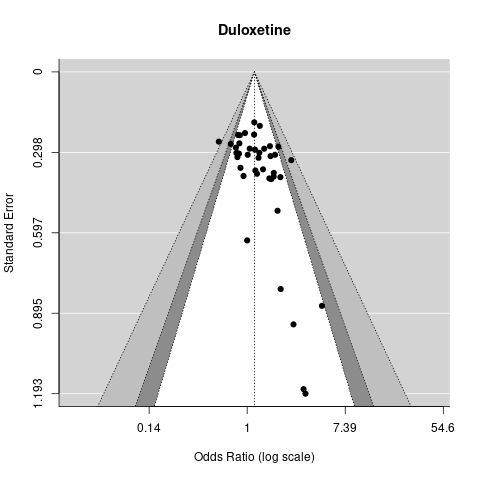
\includegraphics[width=0.5\textwidth]{img/withdrawalduloxetine-placebo-funnel.png}
\caption[Withdrawal by condition: duloxetine]{
Subgroup analysis by condition. \input{img/withdrawal-duloxetine-placebo-rma-caption.txt}
}
\label{fig:withdrawal-dulox-plac}
\end{figure}


Some of the heterogeneity observed in duloxetine compared to placebo trials is explained by differences between pain condition groups (Figure \ref{fig:withdrawal-condition-dulox-plac}), where neuropathic and musculoskeletal patients were more likely to withdraw from the trials than fibromyalgia patients.

\begin{figure}

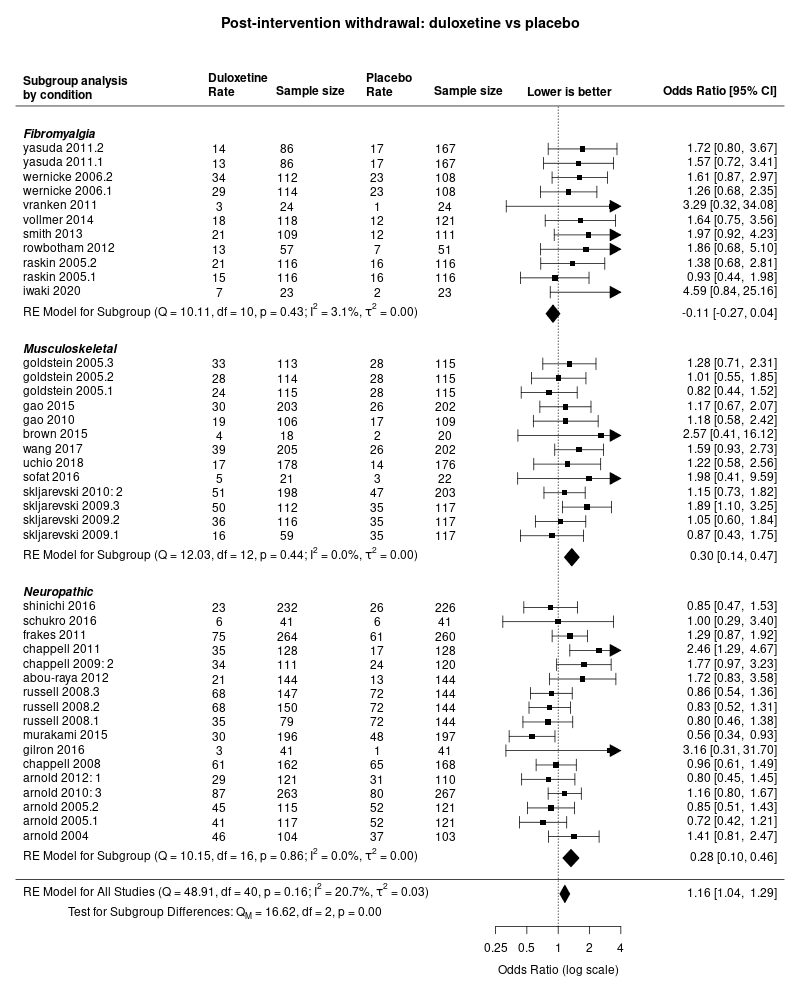
\includegraphics[width=\textwidth]{img/withdrawal-condition-duloxetine-placebo-forest.png}
\caption[Withdrawal by condition: duloxetine]{
Subgroup analysis by condition. \input{img/withdrawal-condition-duloxetine-placebo-rma-caption.txt}
}
\label{fig:withdrawal-condition-dulox-plac}
\end{figure}

Heterogeneity of duloxetine compared with placebo was not explained by risk of bias. However, some heterogeneity is explained by dose, whereby those given high dose more likely to experience withdrawal (Figure \ref{fig:withdrawal-dose-dulox-plac}). Heterogeneity was not explained by duration of study.

\begin{figure}
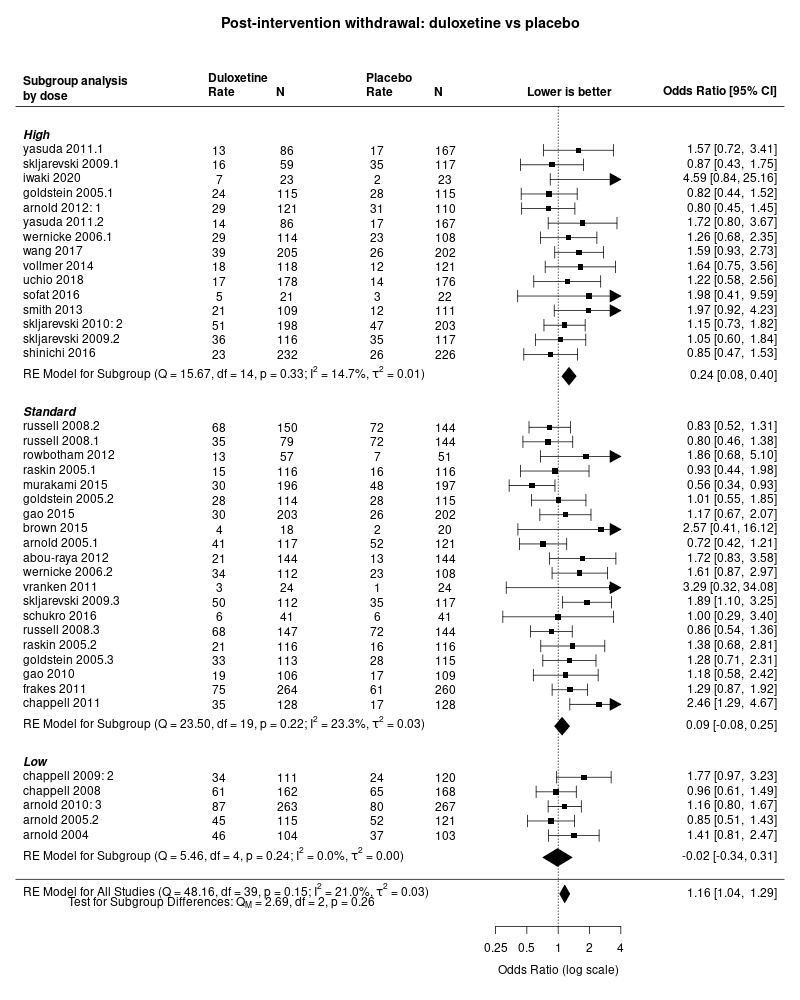
\includegraphics[width=\textwidth]{img/withdrawal-dose-duloxetine-placebo-forest.png}
\caption[Withdrawal by dose: duloxetine]{
Subgroup analysis by dose. \input{img/withdrawal-dose-duloxetine-placebo-rma-caption.txt}
}
\label{fig:withdrawal-dose-dulox-plac}
\end{figure}


\subsubsection{Milnacipran}

Milnacipran observations have very serious risk of bias and some funnel-plot asymmetry (Figure \ref{fig:with-milna-plac}) suggests possible publication bias.

\begin{figure}

\begin{knitrout}
\definecolor{shadecolor}{rgb}{0.969, 0.969, 0.969}\color{fgcolor}\begin{kframe}


{\ttfamily\noindent\bfseries\color{errorcolor}{\#\# Error in include\_graphics("{}img/withdrawal-milnacipran-placebo-forest.png"{}): Cannot find the file(s): "{}img/withdrawal-milnacipran-placebo-forest.png"{}}}\end{kframe}
\end{knitrout}


\caption[Withdrawal, milnacipran]{
\input{img/withdrawal-rob-milnacipran-placebo-rma-caption.txt}
}
\label{fig:with-milna-plac}
\end{figure}



Risk of bias explains some of the heterogeneity in milnacipran observations reporting withdrawal (Figure \ref{fig:withdrawal-rob-dulox-plac}), where studies ranked with low risk of bias were significantly more likely to report higher withdrawal rates.

\begin{figure}
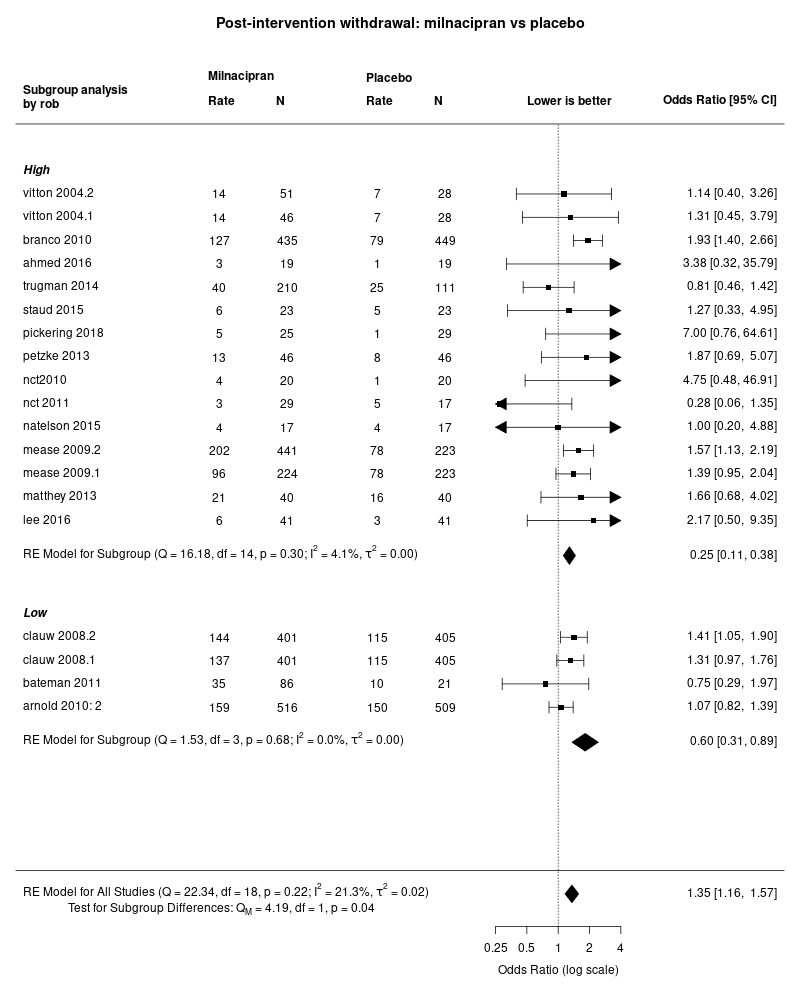
\includegraphics[width=\textwidth]{img/withdrawal-rob-milnacipran-placebo-forest.png}
\caption[Withdrawal ROB: milnacipran]{
Subgroup analysis by rob.
\input{img/withdrawal-rob-milnacipran-placebo-rma-caption.txt}
}
\label{fig:withdrawal-rob-dulox-plac}
\end{figure}

Length of study also explains some of the heterogeneity in withdrawal, with studies lasting more than 12 weeks more likely to report withdrawal (Figure \ref{fig:withdrawal-duration-milna-plac}).

\begin{figure}
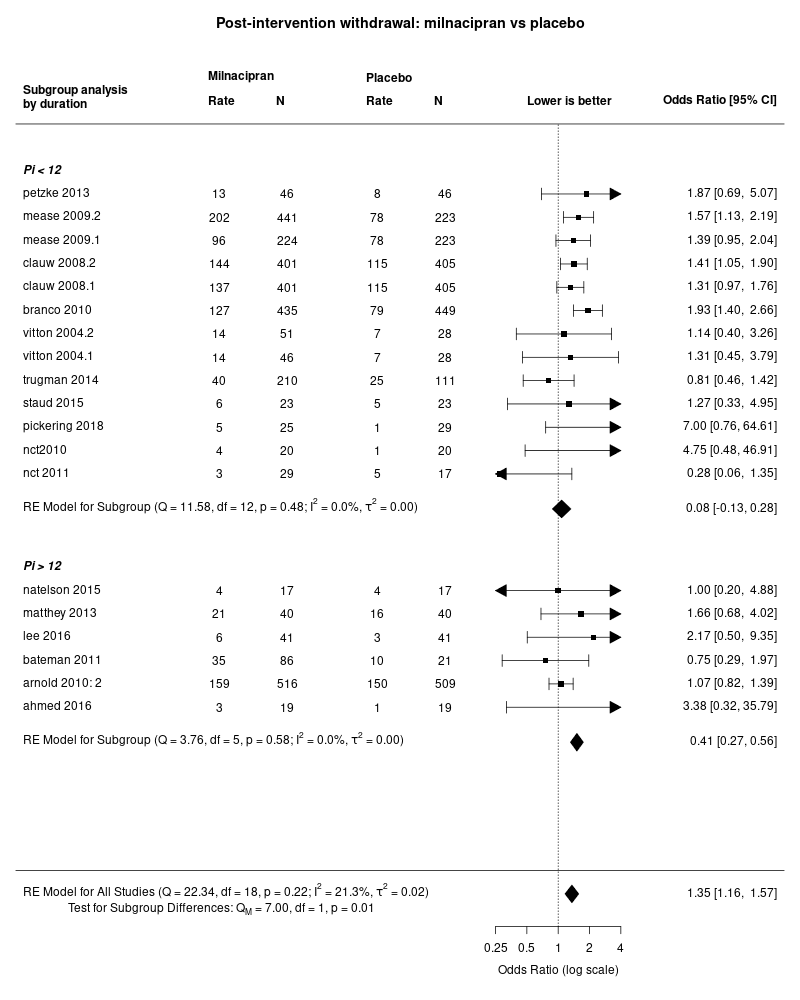
\includegraphics[width=\textwidth]{img/withdrawal-duration-milnacipran-placebo-forest.png}
\caption[Withdrawal duration: milnacipran]{
Subgroup analysis by duration.
}
\label{fig:withdrawal-duration-milna-plac}
\end{figure}

\subsubsection{Amitriptyline}

Amitriptyline showed serious inconsistency and imprecision (Figure \ref{fig:with-amitr-plac}), however little indication of publication bias. Heterogeneity was not explained by risk of bias or duration of study. These observations have very serious risk of bias.


\begin{figure}

\begin{knitrout}
\definecolor{shadecolor}{rgb}{0.969, 0.969, 0.969}\color{fgcolor}
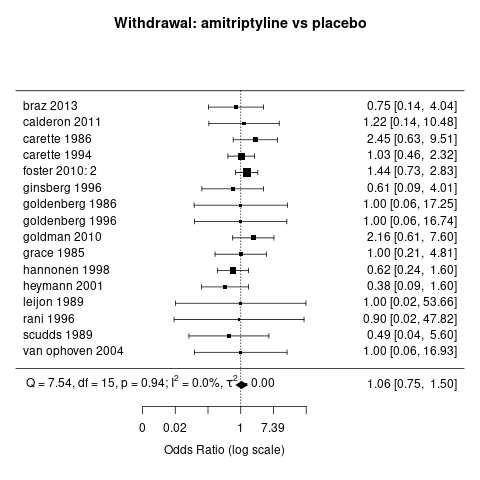
\includegraphics[width=0.5\linewidth,height=0.35\textheight]{img/withdrawal-amitriptyline-placebo-forest} 
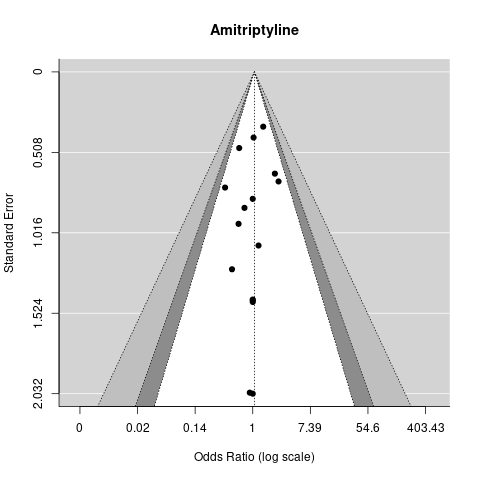
\includegraphics[width=0.5\linewidth,height=0.35\textheight]{img/withdrawal-amitriptyline-placebo-funnel} 
\end{knitrout}

\caption[Withdrawal: amitritpyline vs placebo]{withdrawal-rob-amitritpyline-placebo-rma-captin.txt}
\label{fig:with-amitr-plac}
\end{figure}

\section{Physical functioning (Change scores)}

31 parallel-design studies reported phsycial funcitoning as change score measures, evaluating 15 interventions over a population of 11,472. Studies ran from 6 to 28 weeks, with median length 12 weeks. In addition to trials comparing placebo, there was one study that compared cognitive behavioural therapy and milnacipran, one study that compared duloxetine and pregabalin, and one that compared paroxetine against therapy. This creates the disconnected network shown in Summary of findings Table \ref{tab:physicalcs}.


\soffignew
{physicalcs}
{img/physical-change_score-net.png}
{img/physical-change_score-pico.png}
{img/physical-change_score-sof.png}
{Physical functioning (Change score)}

\textbf{Interventions} (number of studies): Placebo (28); duloxetine (20); milnacipran (4); citalopram (2); abt-894 (1); cbt (1); cbt and milnacipran (1); esreboxetine (1); fluoxetine (1); imipramine (1); mirtazapine (1); nortriptyline (1); paroxetine (1); pregabalin (1); psychotherapy (1); usual treatment (1).

\subsection{Meta-analyses}

\subsubsection{Duloxetine}

Results were not inconsistent or imprecise. Heterogeneity was not explained by condition or dose.

\section{Physical functioning (Post intervention)}

28 studies (5 crossover, 23 parallel) reported physical functioning as post-intervention measures, evaluating 32 interventions over a population of 3424 participants. Studies ran from 2 to 36 weeks, with median length 9 weeks. The network (Table \ref{tab:physicalpi}) is very disconnected. There were three trials that compared amitriptyline to benzotropine mesylate, and 7 further comparators unique to single trials.


\soffignew
{physicalpi}
{img/physical-post_int-net.png}
{img/physical-post_int-pico.png}
{img/physical-post_int-sof.png}
{Physical functioning (Post intervention)}

\textbf{Interventions} (number of studies): Placebo (18); amitriptyline (6); duloxetine (6); benzotropine mesylate (5); fluoxetine (3); pregabalin (3); milnacipran (2); nortriptyline (2); acupuncture (1); benzotropine mesylate + cbt (1); cst (1); cst + sertraline (1); cyclobenzaprine (1); desipramine (1); desipramine + cbt (1); dothiepin (1); epidural injection (1); epidural injection + amitriptyline (1); escitalopram (1); esreboxetine (1); fluoxetine + melatonin (1); gabapentin (1); gabapentin + nortriptyline (1); melatonin (1); mirtazapine (1); moclobemide (1); morphine (1); morphine + nortriptyline (1); paroxetine (1); pregabalin + duloxetine (1); sertraline (1); trazodone (1); venlafaxine (1).


\section{Sleep quality (Change score)}


Sleep was reported as a change-score measure in 17 parallel studies evaluating 4 interventions over a total of 6077 participants. Studies ran from 6 to 52 weeks, with median length 12 weeks. The geometry of the direct-evidence network (Summary of findings Table \ref{tab:sleepcs}) shows all trials compared one intervention with placebo. The participants were mostly fibromyalgia nad neuropathic pain patients.

\soffignew
{sleepcs}
{img/sleep-change_score-net.png}
{img/sleep-change_score-pico.png}
{img/sleep-change_score-sof.png}
{Sleep quality (change score)}

\textbf{Interventions} (number of studies): Placebo (16); duloxetine (13); milnacipran (2); citalopram (1); esreboxetine (1).


\subsection{Meta-analyses}

\subsubsection{Duloxetine}

No serious inconsistency, publication bias, or imprecision was detected. Heterogeneity of duloxetine compared with placebo not explained by condition, risk of bias, or duration of study.

\subsubsection{Milnacipran}

Meta-analsyis results are consistent for milnacipran compared to placebo, and with the network meta-analysis estimates. Some publication bias is suggested by funnel plot asymmetry, however not significant, and these results have high risk of bias. Heterogeneity of results not explained by duration of study.

\section{Sleep quality (post intervention)}

% redo

Sleep was reported as post-intervention measure in 19 studies (6 crossover, 13 parallel) evaluating 23 interventions over a total of 1881 participants. Studies ran from 2 to 24 weeks, with median length 6 weeks. The geometry of the direct-evidence network (Summary of findings \ref{tab:sleeppi}) is disconnected, with various comparators used, each of which unique to one trial, and almost half (9 studies) not including placebo trials.

\soffignew
{sleeppi}
{img/sleep-post_int-net.png}
{img/sleep-post_int-pico.png}
{img/sleep-post_int-sof.png}
{Sleep quality (post intervention)}

\textbf{Interventions}: Placebo (11); amitriptyline (7); duloxetine (5); pregabalin (3); fluoxetine (2); gabapentin (2); milnacipran (2); nortriptyline (2); acupuncture (1); amitriptyline + fluoxetine (1); amitriptyline + splint (1); carbamazepine (1); escitalopram (1); gabapentin + nortriptyline (1); melatonin (1); melatonin + amitriptyline (1); moclobemide (1); morphine (1); nortriptyline + morphine (1); physical therapy (1); pregabalin + duloxetine (1); sertraline (1); venlafaxine (1); waitlist (1).

\subsection{Meta-analyses}

Subgroup anlaysis by dose was not possible.

\subsubsection{Duloxtine}

Meta-analyis results for duloxetine compared to placebo were consistent for both post-intervention and change-score measures within studies and with network meta-analysis estimates. Publication bias is suspected for post intervention results, and change score results have a proportion of 0.4 high risk of bias studies.

\subsubsection{Amitriptyline}

Meta-analysis of amitriptyline compared to placebo was consistent with findings of network meta-analysis estimates. The variation between studies accounts for most of the heterogeneity observed in the trials ($I^2 = 95$\%). Publication bias strongly suspected, as well as high risk of bias.


\section{Quality of life}

Quality of life was reported as post-intervention measures by 17 studies (3 crossover, 14 parallel) evaluating 21 interventions across a total of 2857 participants. The participants were primarily fibromyalgia patients. Studies ran from 6 to 24 weeks, with a median time range of 8 weeks. Most comparisons (see network in Summary of findings \ref{tab:qol}) were between esreboxetine and placebo, as well as duloxetine and placebo. The exceptions being two trials that did not include a placebo trial but instead cognitive behavioural therapy and pregabalin, respectively. The participants were largely fibromyalgia pain patients.


\soffignew
{qol}
{img/qol-post_int-net.png}
{img/qol-post_int-pico.png}
{img/qol-post_int-sof.png}
{Quality of life}

\textbf{Interventions (number of studies)}: Placebo (10); Amitriptyline (6); Duloxetine (5); Fluoxetine (3); Acupuncture (2); Melatonin (2); Milnacipran (2); Pregabalin (2); Abt-894 (1); Amitriptyline + fluoxetine (1); Amitriptyline + splint (1); Benzotropine mesylate (1); Cbt (1); Desipramine (1); Education (1); Esreboxetine (1); Fluoxetine + melatonin (1); Melatonin + amitriptyline (1); Nortriptyline (1); Pregabalin + duloxetine (1); Saffron/crocin (1); Waitlist (1).


\subsection{Meta-analyses}

Most subgroup analyses were not possible. Meta-analyses were of two or three observations, and did not display, given the sparse nature of the plots, any particular outliers.

\subsubsection{Duloxetine}

There was significant difference between quality of life improvement for duloxetine compared to placebo between different pain condition groups (Figure \ref{fig:qolcs-condition-dulox-plac}).

\begin{figure}
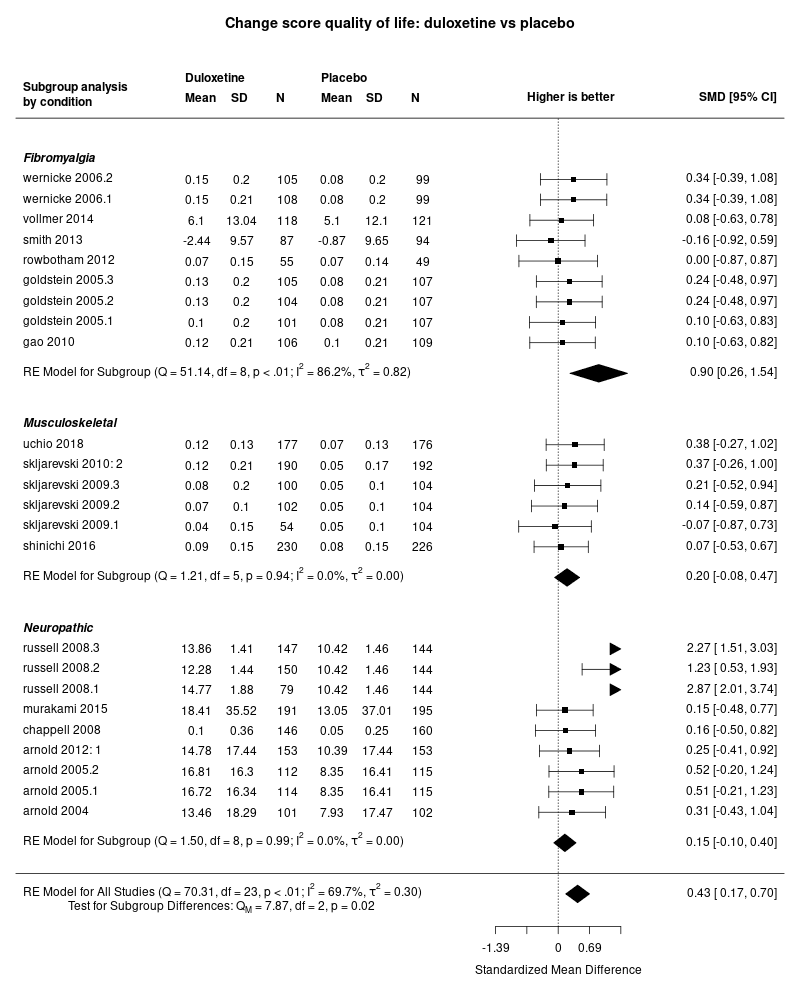
\includegraphics[width=\textwidth]{img/qol-change_score-condition-duloxetine-placebo-forest.png}
\caption[QOL by condition, duloxetine]{
Subgroup anlaysis by condition.
\input{img/qol-change_score-condition-duloxetine-placebo-rma-caption.txt}
}
\label{fig:qolcs-condition-dulox-plac}
\end{figure}

There was not significant difference between low, standard, and high-dose groups, but there is still observable (Figure \ref{fig:qolcs-dose-dulox-plac}) variation between the groups.


\begin{figure}
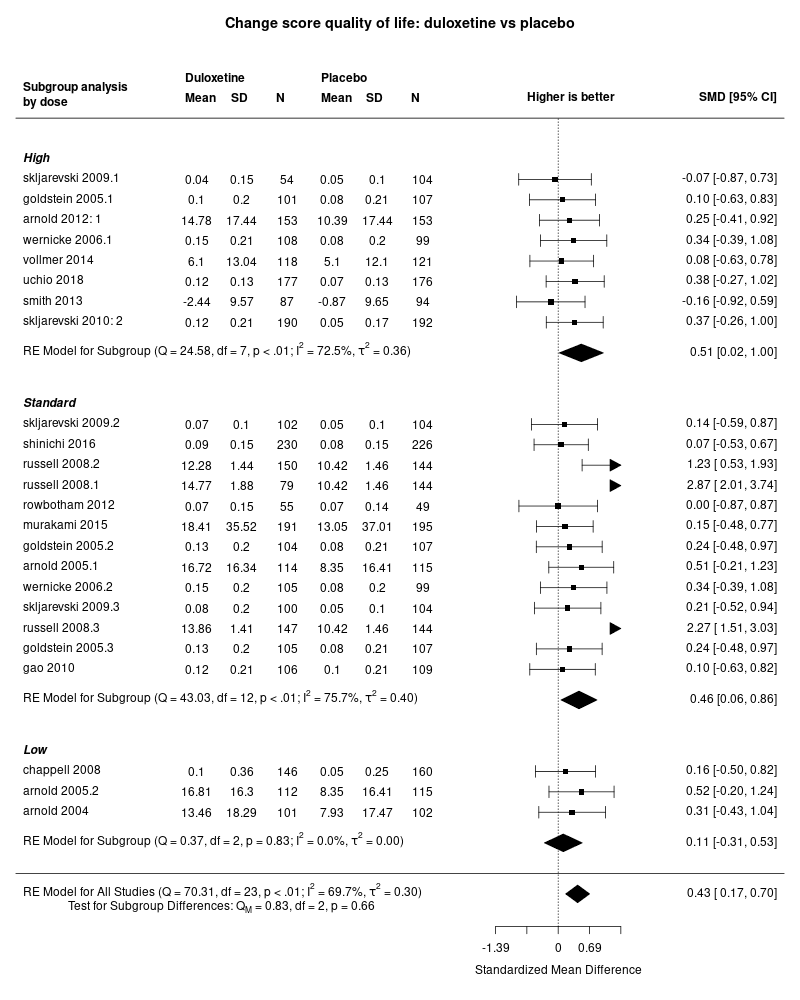
\includegraphics[width=\textwidth]{img/qol-change_score-dose-duloxetine-placebo-forest.png}
\caption[QOL by dose, duloxetine]{
Subgroup anlaysis by dose.
\input{img/qol-change_score-dose-duloxetine-placebo-rma-caption.txt}
}
\label{fig:qolcs-dose-dulox-plac}
\end{figure}

\subsubsection{Milnacipran}

There is some heterogeneity in milnacipran compared to placebo measuring quality of life (Figure \ref{fig:qolcs-dose-milna-plac}).

\begin{figure}
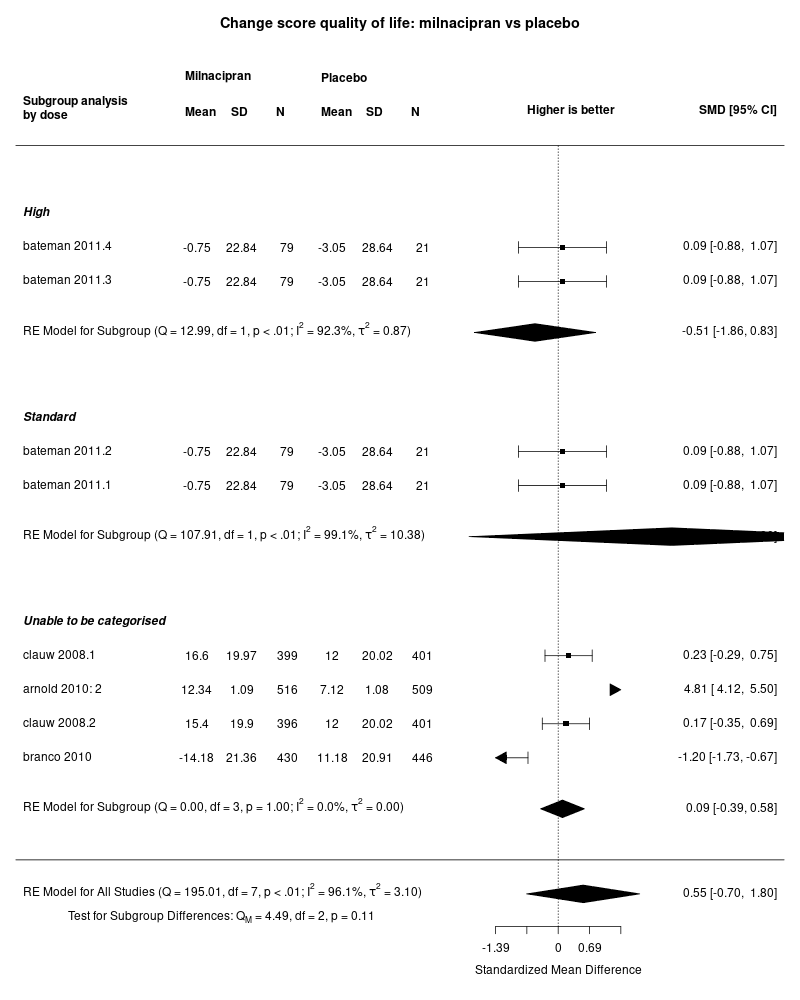
\includegraphics[width=\textwidth]{img/qol-change_score-dose-milnacipran-placebo-forest.png}
\caption[QOL by dose,milnacipran]{
Subgroup anlaysis by dose.
\input{img/qol-change_score-dose-milnacipran-placebo-rma-caption.txt}
}
\labe{fig:qolcs-dose-milna-plac}
\end{figure}

\chapter{Risk of bias summaries}

Figure \ref{fig:rob-bar} shows the distribution of risk of bias for each of the criteria and Figure \ref{fig:rob-grid} shows each study's risk of bias criteria.

\begin{figure}
\centering
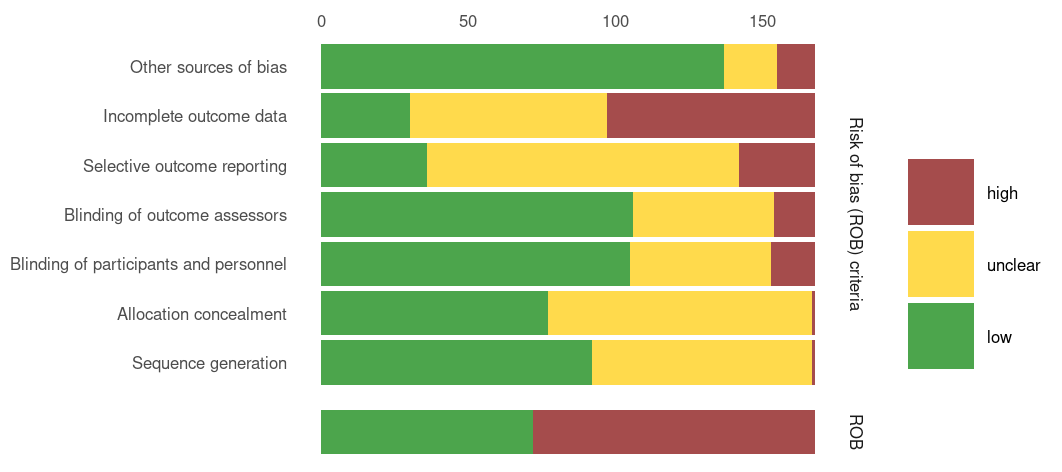
\includegraphics[width = 0.5\textwidth]{img/rob-bar.png}
\caption{Risk of bias distributions for criteria.}
\label{fig:rob-bar}
\end{figure}


\begin{figure}
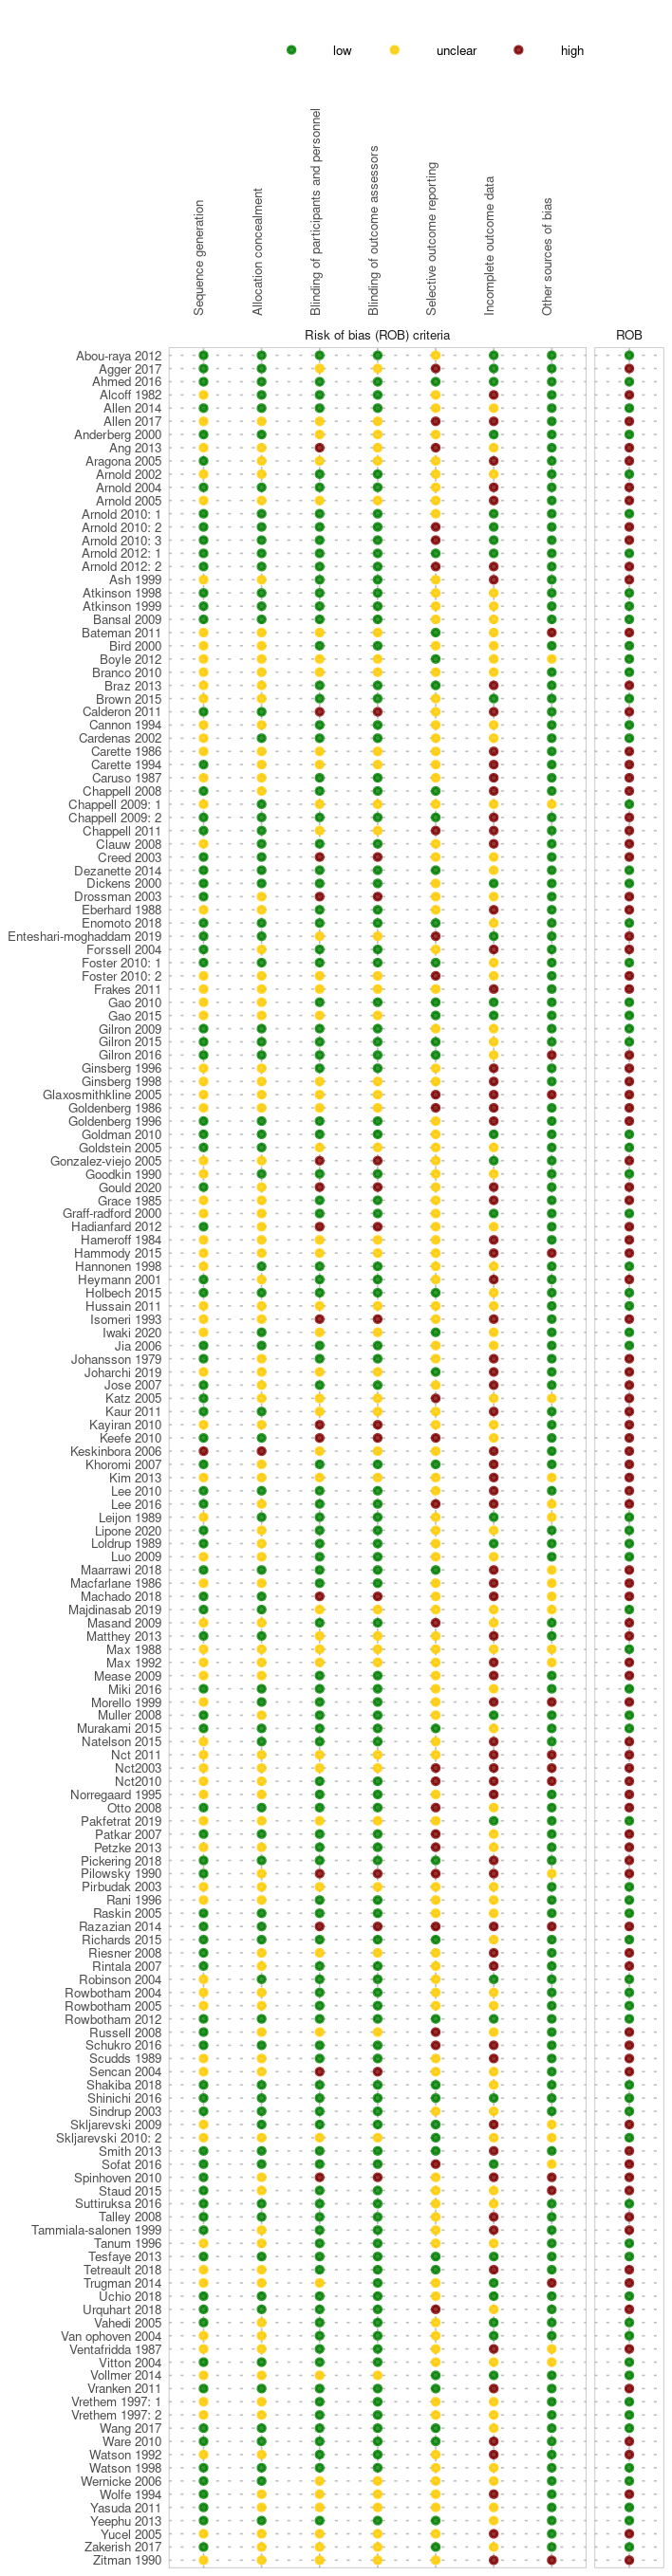
\includegraphics{img/rob-grid.png}
\caption{Risk of bias criteria for studies.}
\label{fig:rob-grid}
\end{figure}
s


\end{document}
